% 
% Systemen voor Online Verkiezingen
% @author Pieter Maene <pieter.maene@student.kuleuven.be>
%

\documentclass[master=elt,masteroption=im,inputenc=utf8]{kulemt}
\setup{title={Online verkiezingen in de praktijk: verbetering en toepassing van het Helios verkiezingssysteem},
  author={Pieter Maene},
  promotor={Prof. dr. ir. B. Preneel},
  assessor={Prof. dr. ir. V. Rijmen \and Prof. dr. ir. L. Van Eycken},
  assistant={Dr. ir. J. Hermans \and Dr. ir. F. Vercauteren}
}

\setup{filingcard,
  translatedtitle={Online Elections in Practice: Improvement and Application of the Helios Voting System},
  udc=621.3,
  shortabstract={
    % 
% Short Abstract
% @author Pieter Maene <pieter.maene@student.kuleuven.be>
%

Een voter-verifiable stemsysteem geeft de kiezer de mogelijkheid om na te gaan of zijn eigen stem correct geregistreerd is en of het resultaat correct is. Het is mogelijk om een dergelijk systeem met papieren stembiljetten te implementeren, zowel met als zonder cryptografische technieken. Helios is een voter-verifiable stemsysteem voor online verkiezingen. De procedure die bij deze systemen gevolgd moet worden, is echter vaak zeer complex. In deze thesis wordt de procedure gegeven die in Helios gevolgd moet worden om een verkiezing op te zetten. De interface van het systeem werd ook herwerkt om de beheerder beter te ondersteunen. Ook de applicatie die gebruikt wordt door de kiezers werd vereenvoudigd. Na het systeem uitgebreid getest te hebben, werd het in de praktijk gebruikt voor een re\"ele verkiezing waarbij ongeveer 750 mensen hun stem uitbrachten. Daarnaast wordt besproken hoe de trustees hun geheime sleutels kunnen bewaren. Er wordt ook onderzocht of de tekstuele fingerprints niet op een betere manier weergegeven kunnen worden. Tot slot worden de prestaties van de Web Cryptography API vergeleken met deze van bestaande implementaties in JavaScript. Deze nieuwe specificatie geeft ontwikkelaars toegang tot cryptografische functies die in de browser ingebouwd zijn.
  }
}

% Kies de fonts voor de gewone tekst, bv. Latin Modern
\setup{font=lm}

% Hier kun je dan nog andere pakketten laden of eigen definities voorzien
\usepackage{amsmath,amssymb,mathtools}
\usepackage{enumitem}
\usepackage{float}
\usepackage{kulemtx}
\usepackage{multirow,bigstrut}
\usepackage[np,autolanguage]{numprint}
\usepackage{pdfpages}
\usepackage{url}

% De optie colorlinks mag verwijderd worden voor de af te drukken versie
\usepackage[pdfusetitle,colorlinks,plainpages=false]{hyperref}

% Verwijder de "%" op de volgende lijn als je de kaft wil afdrukken
%\setup{coverpageonly}

% Customisations
\graphicspath{{./images/}}

\setlength{\parindent}{0pt}
\setlist[description]{topsep=0.5em, itemsep=0.25em, leftmargin=2em, labelindent=2em}

\headstyles{kulemtman}

% Document
\begin{document}

  % Alias
  % 
% Alias
% @author Pieter Maene <pieter.maene@student.kuleuven.be>
%

\renewcommand{\ref}[1]{\mbox{\autoref{#1}}}

\renewcommand{\chapterautorefname}{Chapter}
\renewcommand{\equationautorefname}{Eq.}
\renewcommand{\figureautorefname}{Fig.}
\renewcommand{\footnoteautorefname}{Footnote}
\renewcommand{\itemautorefname}{Item}
\renewcommand{\sectionautorefname}{Section}
\renewcommand{\subsectionautorefname}{Section}
\renewcommand{\subsubsectionautorefname}{Section}
\renewcommand{\paragraphautorefname}{Paragraph}
\renewcommand{\subparagraphautorefname}{Paragraph}
\renewcommand{\pageautorefname}{Page}
\renewcommand{\tableautorefname}{Table}

\newcommand{\cplusplus}{C\texttt{++}\ }

  \begin{preface}
    %
% Preface
% @author Pieter Maene <pieter.maene@student.kuleuven.be>
%

Deze thesis heeft mij de kans gegeven om twee zaken samen te brengen die een belangrijk deel uitgemaakt hebben van mijn studententijd. Enerzijds mijn ingenieursopleiding, waar we opgeleid worden om technische oplossingen te ontwikkelen. Anderzijds studentenvertegenwoordiging, waar ik altijd nauw betrokken bij geweest ben.

\npar Ik zou dan ook graag mijn promotor, professor Preneel, willen bedanken om mij de kans te geven hieraan te werken. Ik wil ook dr. ir. Jens Hermans bedanken voor zijn hulp doorheen het jaar. Hij stond altijd klaar om mijn vragen te beantwoorden. Tot slot zou ik graag professor Rijmen, professor Van Eycken en dr. ir. Fréderik Vercauteren bedanken voor het lezen en evalueren van deze tekst.

\npar Mijn dank gaat ook uit naar het praesidium van de Vlaamse Technische Kring. In de eerste plaats voor het vertrouwen in een nieuw systeem, maar ook voor hun tijd om het systeem uit te testen. In het bijzonder zou ik Robin Ska willen bedanken om de verkiezing te beheren. Ook Dani\"el Slenders, Jeroen Van Hemelen, Tom Van der Voorde en Daan Wendelen verdienen een bijzondere vermelding als trustees.

\npar Tot slot zou ik graag mijn familie en vrienden willen bedanken. Zij hebben mij de voorbije vijf jaar steeds met raad en daad bijgestaan en gesteund in mijn keuzes.
  \end{preface}

  \kulemtmanToC
  \tableofcontents

  \begin{abstract}
    %
% Abstract
% @author Pieter Maene <pieter.maene@student.kuleuven.be>
%

Verkiezingen spelen een belangrijke rol in een democratische maatschappij. Kiezers moeten op een betrouwbare en gebruiksvriendelijke manier hun stem kunnen uitbrengen. Bij de huidige systemen moet de kiezer vertrouwen hebben in de organisatie die verantwoordelijk is voor de verkiezingen. Een voter-verifiable stemsysteem geeft hem de mogelijkheid om na te gaan of zijn eigen stem correct geregistreerd is en of het resultaat correct is.

\npar Het is mogelijk om een dergelijk systeem met papieren stembiljetten te implementeren, zowel met als zonder cryptografische technieken. Helios is een voter-verifiable stemsysteem voor online verkiezingen. De procedure die bij deze systemen gevolgd moet worden, is echter vaak zeer complex.

\npar In deze thesis wordt de procedure gegeven die in Helios gevolgd moet worden om een verkiezing op te zetten. De interface van het systeem werd ook herwerkt om de beheerder beter te ondersteunen in deze procedure. Ook de applicatie die gebruikt wordt door de kiezers werd vereenvoudigd. Na het systeem uitgebreid getest te hebben, werd het in de praktijk gebruikt voor een re\"ele verkiezing waarbij ongeveer 750 mensen hun stem uitbrachten.

\npar Daarnaast worden aanbevelingen gegeven voor de trustees om hun geheime sleutels te bewaren. Er wordt ook onderzocht of de tekstuele fingerprints niet op een betere manier weergegeven kunnen worden. Tot slot worden de prestaties van de Web Cryptography API vergeleken met deze van bestaande implementaties in JavaScript. Deze nieuwe specificatie geeft web ontwikkelaars toegang tot cryptografische functies die in de browser ingebouwd zijn.
  \end{abstract}
  
  \listoffiguresandtables
  
  %TODO Lijst van afkortingen en symbolen
  \chapter{Lijst van afkortingen en symbolen}
  \section*{Lijst van afkortingen}
  \begin{flushleft}
    \renewcommand{\arraystretch}{1.1}
    \begin{tabularx}{\textwidth}{@{}p{12mm}X@{}}
      DRE & Direct-Recording Electronic \\
      VVPAT & Voter-Verified Paper Audit Trail
    \end{tabularx}
  \end{flushleft}
  \section*{Lijst van symbolen}
  \begin{flushleft}
    \renewcommand{\arraystretch}{1.1}
    \begin{tabularx}{\textwidth}{@{}p{12mm}X@{}}
      $pk$ & Publieke sleutel \\
      $sk$ & Geheime sleutel \\
      $df$ & Decryptiefactor
    \end{tabularx}
  \end{flushleft}

  \mainmatter

  % Chapters
  % 
% Inleiding
% @author Pieter Maene <pieter.maene@student.kuleuven.be>
%

\chapter{Inleiding}
\label{chap:inleiding}

Verkiezingen zijn een essentieel onderdeel van het democratisch proces en spelen dus een zeer belangrijke rol in onze maatschappij. In 2014 vinden in 40 landen nationale verkiezingen plaats. 42\% van de wereldbevolking zal dit jaar hun stem kunnen uitbrengen.\cite{news:economist_2014_ballot_boxes} Ook in Belgi\"e is 2014 een groot verkiezingsjaar: op 25 mei werd tegelijk gestemd voor het Europees parlement, de Kamer van volksvertegenwoordigers en de parlementen van de deelstaten.

\npar In 2012 werd tijdens de presidenti\"ele verkiezingen in Amerika door beide kandidaten ongeveer \'e\'en miljard dollar uitgegeven tijdens hun campagne.\cite{news:nytimes_2012_money_race} In Belgi\"e werd tijdens de federale verkiezingen van 2010 door alle partijen samen 13,7 miljoen euro gespendeerd. Niet alleen de budgetten van de kandidaten zijn zo hoog: de kosten van de organisatie worden voor 25 mei op meer dan 10 miljoen euro geschat.\cite{news:tijd_moeder_aller_verkiezingen_kostprijs}

\npar Gezien het belang van de verkiezingen en de enorme bedragen die ermee gemoeid gaan, is het dus noodzakelijk dat er een betrouwbaar systeem is om het resultaat vast te leggen. Het moet bovendien eenvoudig te gebruiken zijn door de kiezers. Tijdens de Amerikaanse presidentsverkiezingen van 2000 werd in Palm Beach County, Florida een biljet gebruikt dat verwarrend zou zijn. Dit kreeg des te meer aandacht omdat de uitslag erg nipt was.\cite{wiki:united_states_presidential_election_in_florida_2000} In Belgi\"e stemt bijna de helft van de kiezers elektronisch, maar ook hier kan de interface voor problemen zorgen. Tijdens de gemeenteraadsverkiezingen van 2012 kon per ongeluk een voorkeurstem gegeven worden door te lang op het scherm te duwen.\cite{news:maddens_zijn_de_stemcomputers_wel_te_vertrouwen} In veel steden werden voor 25 mei stemcomputers ter beschikking gesteld om op te oefenen.\cite{news:de_redactie_ga_eens_oefenen_op_een_stemcomputer}

\npar Het is dus niet eenvoudig om een gebruiksvriendelijke oplossing te ontwikkelen, noch voor papieren biljetten, noch wanneer digitaal gestemd wordt. Daarnaast heeft de kiezer vandaag geen enkele manier om na te gaan of zijn stem juist meegeteld is en of het algemene resultaat correct is. Hij moet de instantie die de verkiezing organiseert dus volledig vertrouwen. Dit kan opgelost worden door gebruik te maken van een voter-verifiable systeem. Een groot nadeel is echter dat veel van deze systemen een complexe procedure hebben. Helios is een systeem dat het mogelijk maakt om online voter-verifiable verkiezingen te organiseren.

\npar In \ref{chap:literatuurstudie} worden papieren systemen besproken die voter-verifiable zijn. Veel van de technieken die hier gebruikt worden, zullen ook terugkomen in Helios. \ref{chap:helios} tot \ref{chap:interface} behandelen de werking van dit systeem, de procedure die gevolgd moet worden voor het opzetten van een verkiezing en de wijzigingen aan de interface. Het aangepaste systeem werd ook in de praktijk gebruikt om na te gaan hoe bruikbaar het is voor een echte verkiezing (\ref{chap:kringverkiezing}). 

\npar In \ref{chap:sleutels_en_fingerprints} wordt kort gekeken naar methoden om de sleutels en fingerprints te bewaren. Tot slot worden de prestaties van de Web Cryptography API ge\"evalueerd (\ref{chap:web_cryptography_api}).

  
  % 
% Literatuurstudie
% @author Pieter Maene <pieter.maene@student.kuleuven.be>
%

\chapter{Literatuurstudie}
\label{chap:literatuurstudie}

Deze thesis handelt over methoden voor online verkiezingen. Een interessant verwant probleem zijn systemen die gebruik maken van papier. Eerst wordt een kort overzicht van de geschiedenis van stemsystemen gegeven (\ref{sec:ls:geschiedenis}). Vervolgens worden de belangrijkste vereisten bekeken waaraan deze systemen moeten voldoen (\ref{sec:ls:vereisten}). Belangrijk hierbij is de definitie van een voter verifiable systeem. Tot slot onderzoeken we zowel systemen die geen gebruik maken van cryptografische methoden (\ref{sec:ls:systemen_zonder_cryptografie}) als deze die daar wel op steunen (\ref{sec:ls:systemen_met_cryptografie}).

\section{Geschiedenis~\cite{adida_advances_in_cryptographic_voting_systems}}
\label{sec:ls:geschiedenis}

Onze samenleving heeft een rijke geschiedenis van stemprocedures, die teruggaat tot Athene in het oude Griekenland. Hier bracht men een negatieve stem uit op een potscherf. In deze paragraaf bekijken we kort enkele die bepalend zijn geweest voor de manier waarop we vandaag werken.\cite{wiki:ostracon}

\npar Sinds de uitvinding van het geheime stembiljet in 1858 in Australi\"e is er eigenlijk niet meer zoveel veranderd. In dit systeem worden de biljetten op voorhand gedrukt door de staat en veilig bewaard tot op de stemdag. Elke stemgerechtigde krijgt op de stemdag een biljet waarna hij zijn stem uitbrengt in een stemhokje. Het grootste voordeel van deze methode ligt in het feit dat elke stem geheim is.

\npar Deze stemmethode maakte het daarnaast ook mogelijk om mechanische (en later elektrische) machines te gebruiken. Mechanische systemen werden gebruikt in grotere gemeenschappen en waren gebaseerd op hendels en mechanische tellers. De eerste van deze machines werden in 1892 ingevoerd in New York. Rond 1960 werden de eerste elektrische machines ingevoerd. Deze maakten gebruiken van optische scans. Bij deze systemen moet de stem meestal op een specifieke manier aangegeven worden, bijvoorbeeld door het inkleuren van bolletjes.

\npar Sinds 2000 worden Direct Recording by Electronics (DRE) machines steeds vaker gebruikt. Hierop draait speciale stemsoftware, die de keuze van de kiezer digitaal vastlegt. Deze machines maken het stemproces aanzienlijk eenvoudiger. Het grootste probleem is dat er geen enkele bevestiging aan de kiezer gegeven wordt en dat hij deze machines dus volledig moet vertrouwen.\cite{wiki:dre_voting_machine}

\npar Het gebrek aan controle door de kiezer bij DRE vormde de aanleiding voor het ontwerpen van Voter-Verified Paper Audit Trails (VVPAT) machines. Hierbij toont de machine de kiezer een afgeschermde afdruk van zijn stem, waarna hij deze kan accepteren of weigeren. Op die manier kan de kiezer verifi\"eren dat zijn stem correct is. In principe zouden bij een hertelling dan ook deze papieren tickets en niet de digitale data gebruikt moeten worden.\cite{wiki:vvpat}

\section{Vereisten}
\label{sec:ls:vereisten}

Bij het ontwerpen van een stemsysteem zijn er twee tegenstrijdige doelen. Enerzijds moet het mogelijk zijn dat zowel de kiezer thuis kan controleren of zijn stem juist meegeteld is. Anderzijds mag diezelfde persoon niet kunnen bewijzen voor wie hij precies gestemd heeft, noch mag het mogelijk zijn dat anderen hierachter kunnen komen. Wanneer hij dit wel kan, zou hij zijn stem kunnen verkopen aan iemand die de verkiezing wil beïnvloeden, of hiertoe gedwongen worden.

\npar Hoewel het vaak zeer moeilijk is om een grote verkiezing doorslaggevend te wijzigen, wordt stemfraude toch regelmatig geconstateerd.\cite{adida_advances_in_cryptographic_voting_systems} E\'en van de grote moeilijkheden is dat zowel kiezers als bijzitters corrupt kunnen zijn. Er kan dus van geen enkele deelnemer verwacht worden dat hij eerlijk is.

\subsection{Vertrouwen}
\label{sec:ls:vertrouwen}

De huidige manier van stemmen vereist dat de kiezer zeer veel vertrouwen legt in het gebruikte systeem. Zoals verder besproken wordt (\ref{sec:ls:end_to_end_verifiability}), zijn er nieuwe ontwerpen waarbij de kiezer kan controleren of zijn stem correct meegeteld is. Deze systemen steunen vaak op moeilijke cryptografische technieken, die heel wat achtergrondkennis vragen om ze te begrijpen.

\npar Een vereiste voor om het even welk stemsysteem is dat het vertrouwd wordt door een gemiddelde kiezer, de bijzitters, de publieke opinie en media. Opdat deze mensen een dergelijk systeem zouden vertrouwen, moeten de experts die het systeem goedkeuren dit op een eenvoudige manier aan hen kunnen uitleggen.\cite{randell_ryan_voting_technologies_and_trust} Daarom zullen eenvoudige systemen die geen gebruik maken van cryptografie waarschijnlijk sneller aanvaard worden door een breed publiek.

\subsection{End-to-End Verifiability}
\label{sec:ls:end_to_end_verifiability}

In een end-to-end verifiably voting systeem wordt niet nagegaan of de code van de stemmachines volledig correct is. In plaats daarvan wordt wiskundig bewezen dat het resultaat correct is. Op die manier kan de moeilijke en vaak ondoorzichtige fysische chain-of-custody vermeden worden. Dit betekent ook dat iemand niet langer speciale toegang moet hebben om de resultaten te controleren. Om het even wie kan nagaan of de bewijzen correct zijn.

\npar Dergelijke end-to-end verifiable systemen kunnen zowel met als zonder cryptografische technieken gerealiseerd worden. Cryptografie kan enerzijds gebruikt worden om stemmen te encrypteren, zodat ze zeker geheim blijven. Anderzijds geven sommige systemen een zero-knowledge bewijs dat aangetoont dat de stemmen correct geteld zijn.

\section{Systemen zonder cryptografie}
\label{sec:ls:systemen_zonder_cryptografie}

In deze paragraaf worden enkele systemen besproken waarin geen gebruik gemaakt wordt van cryptografie. Open Counting (\ref{sec:ls:open_counting}) is een techniek waarbij alleen de telfase aangepast wordt. Floating receipts (\ref{sec:ls:floating_receipts}) kunnen de veiligheid van elk papieren stemsysteem sterk verbeteren. ThreeBallot (\ref{sec:ls:scratch_card}) en Scratch-Card zijn beiden voter-verifiable systemen die gebruik maken van papieren tickets. Twin (\ref{sec:ls:twin}) bouwt verder op respectievelijk floating receipts. Vooral ThreeBallot wordt in detail besproken omdat de belangrijkste concepten van papier-gebaseerde voter-verifiable verkiezingen hierin aan bod komen.

\subsection{Open Counting~\cite{adi_schuler_frohlich_open_counting}}
\label{sec:ls:open_counting}

Open counting vertrekt van de systemen zoals we ze vandaag kennen, maar de stemmen worden op een nieuwe manier geteld. Het stembiljet is aangepast om eenvoudig optisch geteld te worden. De stemmen worden nog steeds geteld door ambtenaren. Elke stem wordt op een scherm getoond aan verschillende telstations, elk met hun eigen hardware die het getoonde biljet filmt en analyseert. Ieder station geeft op regelmatige tijdstippen zijn huidig totaal en wanneer er onenigheid is, wordt het gedisputeerde biljet gezocht en het probleem opgelost.

\npar Tijdens het tellen geeft ieder station ook een hash van hun opgenomen video. Hiervoor wordt een veilige hash-functie gebruikt. Deze hashes kunnen dan later gebruikt worden tijdens een geautomatiseerde audit om te controleren of er niet geknoeid is met de beelden. Dit proces is publiek en dus kan iedereen zijn eigen hardware meebrengen en de telling zelf uitvoeren. Het systeem wordt zo ontworpen dat een eenvoudige camera en computer volstaan. Ook deze waarnemers kunnen een hash van hun video publiceren om geloofwaardiger over te komen.

\npar De verschillende telstations controleren continu elkaar en ook de waarnemers kunnen achteraf onregelmatigheden melden. Omdat het systeem snel werkt, kan de telling in het stembureau zelf gehouden worden. Op die manier kunnen alle belanghebbenden aanwezig zijn en kan het transport van de ongetelde biljetten vermeden worden. Het transparante karakter en het gebruik van eenvoudige hardware kunnen het vertrouwen van kiezers in het systeem sterk vergroten.

\npar Open counting is een relatief eenvoudige manier om de telprocedure transparanter te maken naar de kiezers. Elke stem moet echter afzonderlijk getoond worden, waardoor dit systeem alleen gebruikt kan worden wanneer het aantal biljetten beperkt is.

\subsection{Floating Receipts~\cite{rivest_smith_three_voting_protocols}}
\label{sec:ls:floating_receipts}

Floating receipts zijn een waardevolle toevoeging voor elk voter-verifiable papieren telsysteem. Een doos met stembiljetten wordt aan de uitgang van het stembureau geplaatst. De kiezer maakt bij het buitengaan een kopie van een stembiljet dat hij hieruit trekt, vooraleer hij zijn eigen erbij legt. Hij neemt dus een willekeurig ticket mee dat niet het zijne is, maar hij kan dit ticket toch later gebruiken om te controleren of de stemprocedure correct verlopen is. Omdat de doos initieel leeg is, krijgen de eerste $T$ kiezers geen ticket mee naar huis. Hierbij is $T$ een constante die veel kleiner is dan het aantal kiezers, maar voldoende groot zodat $1/T$ klein is.

\npar Niemand weet dus met grote waarschijnlijkheid van wie hij het biljet gekopieerd heeft. Omdat de aanvaller geen betrouwbare methode heeft om alle kopie\"en van een ticket te bemachtigen, is het systeem bestendig tegen het vervangen van biljetten of het verkopen van een stem. Een nadeel is dat kiezer niet langer zijn eigen ticket heeft en dus misschien minder gemotiveerd is om te controleren of dit correct meegeteld is. Er wordt echter verondersteld dat een groot aantal kiezers dat toch nog steeds zal doen.

\npar Om floating receipts te gebruiken, moeten de kiezers een extra stap volgen in de stemprocedure. De stemprocedure wordt dus complexer, maar dit kan verantwoord worden door de voordelen die deze techniek met zich meebrengt.

\subsubsection{Short Ballot Assumption}
\label{sec:ls:short_ballot_assumption}

Bij de \textit{Short Ballot Assumption} (SBA) moet het aantal kandidaten op het biljet beperkt blijven. Wanneer er minder mogelijkheden zijn om een biljet in te vullen, wordt de kans kleiner dat iemand anders zijn biljet op identiek dezelfde manier invult. Het wordt dan voor een aanvaller moeilijker om een biljet aan een specifieke kiezer te koppelen.\cite{cichon_kutylowski_weglorz_short_ballot_assumption}

\subsubsection{Twin~\cite{rivest_smith_three_voting_protocols}}
\label{sec:ls:twin}

Twin is een voter-verifiable uitbreiding van het klassieke systeem die gebruik maakt van floating receipts. Een traditioneel stembiljet wordt door elke kiezer individueel ingevuld. Onderaan het stembiljet wordt een ID geplaatst, maar dit wordt verborgen door een kraslaag. Na het invullen wordt het biljet gecontroleerd door een machine die deze laag eraf haalt en het biljet in een doos deponeert. Alle kiezers na de $T^{de}$ krijgen een ticket van een willekeurig biljet mee naar huis. Wanneer de stemming afgelopen is, worden alle verzamelde biljetten gepubliceerd op een bulletin board.

\npar Twin is een heel eenvoudig systeem, zonder ingewikkelde wiskunde of specifieke regels voor het correct invullen van het stembiljet. Aangezien het ticket een kopie is van het biljet van iemand anders, kan een kiezer zijn stem niet verkopen. Daarnaast is het zowel voor de tellers als een aanvaller moeilijk om het resultaat ingrijpend te veranderen zonder gedetecteerd te worden. Er wordt immers verondersteld dat een groot aantal kiezers nagaat of zijn ticket correct op het bulletin board staan.

\npar Het voordeel bij dit systeem is dat het gekende biljet behouden blijft. De kiezer moet dus geen nieuwe regels volgen bij het invullen ervan. Het is echter wel belangrijk dat de kiezer de procedure volgen. Dit moet duidelijk aangegeven worden door de bijzitters.

\subsection{ThreeBallot~\cite{rivest_threeballot}}
\label{sec:ls:threeballot}

ThreeBallot is een stemsysteem dat ontworpen werd door Ronald Rivest in 2006. Het systeem maakt gebruik van een speciaal stembiljet dat bestaat uit drie identieke delen. Er wordt gestemd door het invullen van rijen en het deponeren van kolommen. Door alle stembiljetten samen met een lijst van de kiezers op een publieke website (het bulletin-board) te plaatsen, wordt het systeem end-to-end verifiable.

\subsubsection{Multi-Ballot}
\label{sec:ls:multi-ballot}

De drie delen waaruit het stembiljet bestaat, kunnen ofwel op één blad geprint worden ofwel op meerdere met perforaties ertussen. De drie delen zijn identiek, op een willekeurige identifier na. De drie IDs op een multi-ballot hebben bovendien geen enkel verband met elkaar of met deze op de andere. In \ref{fig:ls:threeballot} wordt een voorbeeld van een multi-ballot getoond.

\begin{figure}
  \center{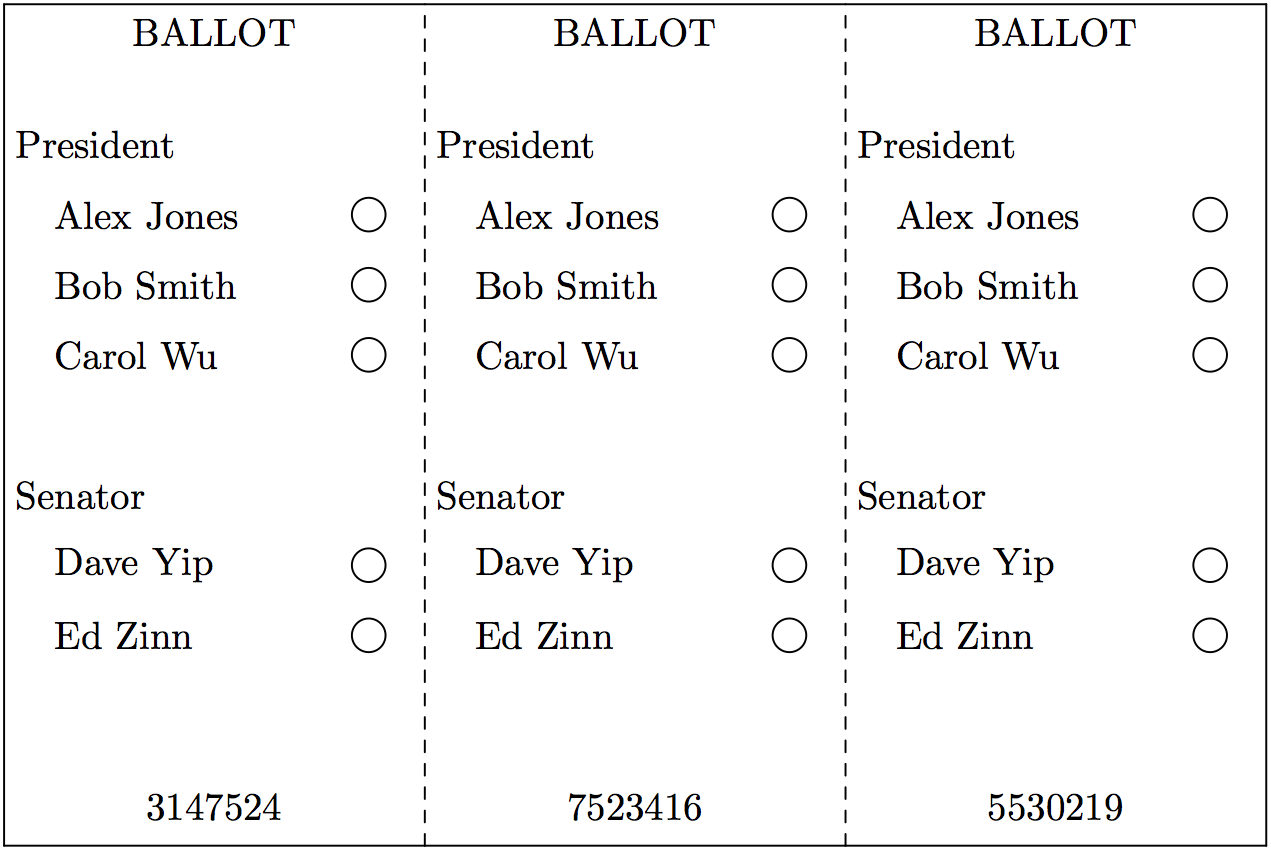
\includegraphics[width=0.5\linewidth]{ls/threeballot.png}}
  \caption{Multi-Ballot\cite{rivest_threeballot}}
  \label{fig:ls:threeballot}
\end{figure}

\npar Bij het invullen van het multi-ballot gelden de volgende regels. Elke rij van drie bolletjes komt overeen met \'e\'en kandidaat. Om voor een kandidaat te stemmen, moet de kiezer exact twee bolletjes inkleuren. Om tegen te stemmen, moet er \'e\'en bolletje aangeduid worden. In elke rij moet exact \'e\'en of twee bolletjes ingevuld zijn, anders is het biljet ongeldig. Hoe de verschillende delen ingevuld zijn, maakt hierbij niet uit.

\npar Omdat het belangrijk is voor de telling dat de kiezer deze regels juist volgt, moet hij na het invullen van het biljet dit invoeren in een controlemachine. Wanneer het biljet niet correct ingevuld is, dan geeft de machine aan waar de kiezer een fout gemaakt heeft. Indien alles wel juist is aangeduid, dan wordt een rode streep geprint op het biljet waarna hij de aparte delen indient. Deze controlemachine mag geen enkele opname maken van de ingevoerde biljetten.

\npar Voordat hij de drie aparte biljetten afgeeft, moet de kiezer er willekeurig \'e\'en uitkiezen waarvan hij een kopie meekrijgt als ticket. Het is het veiligste om dit te implementeren in de controlemachine. Door de manier waarop het biljet ingevuld is, geeft het ticket geen informatie over hoe de kiezer gestemd heeft.

\subsubsection{Tellen van de stemmen}

Wanneer de verkiezing afgelopen is, worden alle biljetten gescand en de gegevens op het bulletin board gepost. Merk op dat het eigenlijke biljet niet online gezet wordt, omdat de kiezer hier iets op zou kunnen schrijven. Ook een lijst van iedereen die deelgenomen heeft aan de stemming wordt ge\"upload. Een kiezer kan nu nagaan of zijn ticket ook op het bulletin board staat.

\npar Omdat alle stemmen op het bulletin board staan, kan iedereen zelf de telling verifi\"eren. De stemmen kunnen zoals anders geteld worden, zij het met een kleine aanpassing. Omdat er twee bolletjes gekleurd zijn bij een voorstem en maar \'e\'en bij een tegenstem, is het resultaat voor elke kandidaat vermeerderd met het aantal kiezers.

\subsubsection{Integriteit}
\label{sec:ls:integriteit}

Door het toevoegen van een ticket en het bulletin board kan de kiezer nagaan dat zijn stembiljet gepubliceerd is en dat het totale aantal geregistreerde biljetten klopt. Deze nieuwe controles zullen ons toelaten om verschillende vormen van fraude eenvoudig te detecteren. Het is ook belangrijk te kijken of zij zelf geen nieuwe zwakheden introduceren.

\npar Het toevoegen van nieuwe stemmen is onmogelijk zonder ook de lijst met kiezers aan te passen. Daarnaast kunnen er ook geen stemmen bijgewerkt of verwijderd worden zonder dat er mogelijk een kiezer komt klagen dat zijn stem niet correct online staat. Grootschalige fraude wordt op deze manier onmogelijk.

\npar Bij de \textbf{Three-Pattern} aanval, vraagt de koper aan de kiezer om alle drie de delen in een bepaald patroon in te vullen. Wanneer hij dit patroon dan niet terugvindt op het bulletin board, wordt de kiezer niet betaald. Een mogelijke oplossing is het gebruik van een DRE machine. Deze print zelf de deelbiljetten in een willekeurig patroon nadat de kiezer zijn keuze gemaakt heeft op een scherm.

\npar Bemerk tot slot dat de controlemachine die de geldigheid van de tickets nagaat zeer goed getest moet worden. Wanneer deze aangepast zou worden, kan ze bijvoorbeeld kiezers toelaten om voor een bepaalde kandidaat drie bolletjes te kleuren en voor een andere geen. Zo zouden die stemmen veel meer gewicht krijgen dan deze die zich wel aan de regels houden. Het is bovendien onmogelijk om dergelijke ongeldige patronen achteraf terug te vinden omdat de verschillende biljetten los van elkaar worden ingediend.

\npar Tot slot zou een aanvaller kunnen betalen voor het ticket van de kiezer. Zo kan deze de correctheid van zijn stem niet meer nagaan. De aanvaller zou dan in theorie het biljet kunnen aanpassen dat op het bulletin board geplaatst werd. De kiezers moeten dus aangemoedigd worden om hun ticket niet af te geven. Deze aanval kan eenvoudig tegengegaan worden wanneer de kiezer zonder medeweten van de aanvaller een kopie maakt van het ticket. Voor een digitaal getekend ticket (bv. met een barcode) volstaat dit namelijk ook om klacht neer te leggen.

\subsubsection{Stemgeheim}

Zoals eerder aangehaald, bevat het ticket zelf geen informatie over hoe de kiezer gestemd heeft. Het mag echter ook niet mogelijk zijn om de drie deelbiljetten aan elkaar te linken. Het ID op het ticket zou anders gebruikt kunnen worden om uit te zoeken welk tripel van een bepaalde kiezer is. Een vereiste voor het systeem is ook dat niemand vooraf weet welke drie deelbiljetten zullen samenhoren. Een mogelijke oplossing hiervoor is om de delen apart te houden en er willekeurig drie te laten trekken door de kiezer.

\npar De kiezer mag zijn eigen multi-ballot niet kunnen reconstrueren op basis van de biljetten die op het bulletin board gepost worden. Dit kan opgelost worden door het ID te printen in de vorm van een 1D of 2D barcode, wat moeilijk te onthouden is. Het is ook verstandig om de kiezer geen vrije toegang te geven tot een kopieermachine bij het maken van het ticket. Dit is de reden dat het ticket best geprint wordt door de controlemachine.

\npar Het moet ook onmogelijk zijn voor de kiezer om zijn stem nog te wijzigen nadat ze aanvaard is door de controlemachine. Een eerste oplossing is om hem geen fysische toegang meer te geven tot de biljetten nadat ze gecontroleerd zijn. Een tweede is om samen met de rode streep (\ref{sec:ls:multi-ballot}) een checksum op het biljet te printen die moeilijk veranderd kan worden door de kiezer.

\npar Tot slot moet er opgepast worden dat een \textbf{Reconstructie} aanval niet mogelijk is. Hierbij haalt een aanvaller alle mogelijke geldige multi-ballots uit de biljetten die op het bulletin board geplaatst werden. Samen met het ticket van de kiezer zou hij dan in sommige gevallen kunnen achterhalen hoe deze gestemd heeft. Om de integriteit van de stemming te kunnen controleren, heeft de kiezer alleen het ticket van een geldig biljet nodig. Het is dus niet noodzakelijk dat hij het ticket van zijn eigen biljet mee naar huis neemt. Een mogelijke manier om dit te implementeren is door gebruik te maken van floating receipts (\ref{sec:ls:floating_receipts}). Deze wordt niet expliciet vermeld in de paper van Rivest, maar hij bespreekt wel gelijkaardige methoden.\cite{rivest_threeballot}

\subsubsection{Bruikbaarheid}

Het ThreeBallot systeem is veel complexer dan de manier waarop nu gestemd wordt. De belangrijkste manier om ervoor te zorgen dat het systeem goed werkt is dan ook het opleiden van de kiezer. Het is ook moeilijker om het biljet te corrigeren wanneer er een fout gemaakt wordt: meestal is de enige optie om opnieuw te beginnen met een blanco biljet. Het gebruik van DRE machine zou het stemmen ook sterk vereenvoudigen. De kiezer moet dan wel controleren dat het geprinte biljet correct is. In \ref{sec:ls:integriteit} werd reeds aangegeven dat dit ook de ThreePattern aanval onmogelijk maakt.

\npar Tot slot merken we nog op dat het tellen van de stemmen wel meer werk vraagt, aangezien er drie keer zoveel biljetten geteld moeten worden. ThreeBallot vergroot het vertrouwen van de kiezer in de integriteit van de verkiezing, ten koste van een moeilijker stemproces en meer werk bij het tellen.

\subsection{Scratch-Card}
\label{sec:ls:scratch_card}

Scratch-Card\cite{randell_ryan_voting_technologies_and_trust} maakt gebruik van een speciaal biljet dat makkelijk in twee gedeeld kan worden (\ref{fig:ls:scratch-card}). Belangrijk is dat de kandidaten op elk biljet in een willekeurige volgorde moeten staan. Een kiezer moet een willekeurig biljet trekken. Na het stemmen moet de kiezer het linkerdeel vernietigen. Hij kan een kopie van het rechterdeel als ticket mee naar huis nemen.

\begin{figure}
  \center{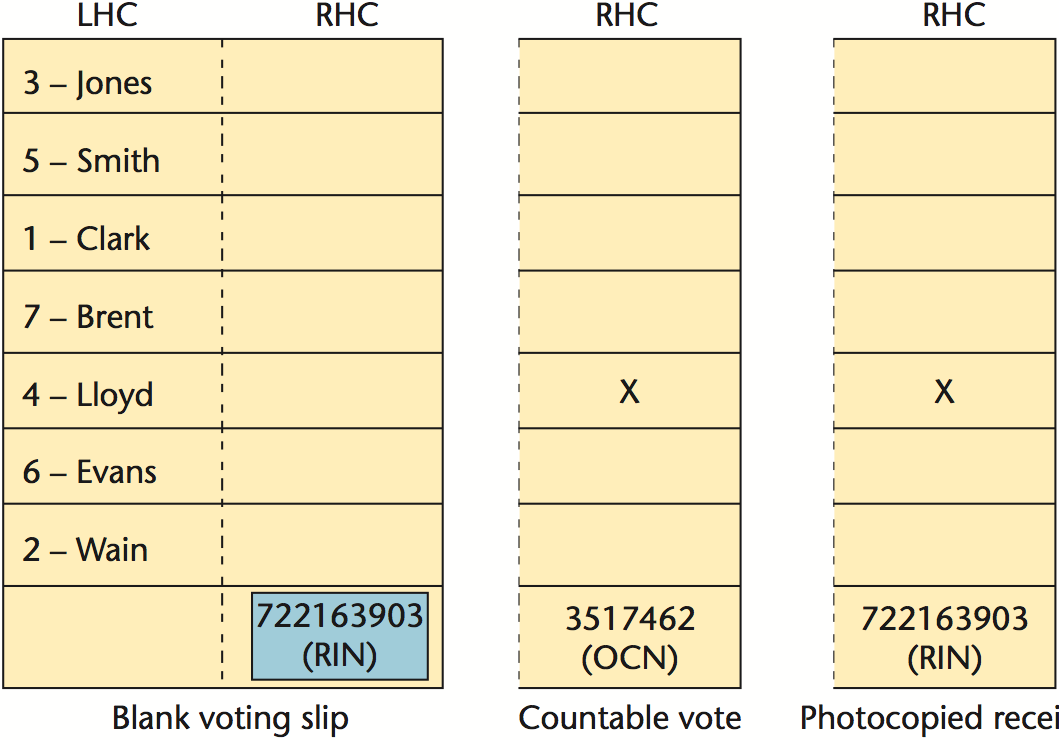
\includegraphics[width=0.5\linewidth]{ls/scratch-card.png}}
  \caption{Scratch-Card biljet\cite{randell_ryan_voting_technologies_and_trust}}
  \label{fig:ls:scratch-card}
\end{figure}

\npar Op het rechterdeel van het biljet is onderaan een kraslaag aangebracht. Bovenop deze laag is het unieke ID (RIN) van het biljet geprint, dat de kiezer later kan gebruiken om zijn stem op het bulletin board terug te controleren. Bovendien verbergt deze laag een vooraf geprinte code die de volgorde van de kandidaten aangeeft (OCN). Bij het tellen wordt deze laag verwijderd en tegelijk verdwijnt ook het RIN van het biljet. Het is zeer belangrijk dat de RIN en OCN volledig ongecorreleerd zijn, want anders zou achterhaald kunnen worden van wie de stem is.

\npar Omdat het ticket een kopie is van het biljet met het kraslaagje nog intact, kan de OCN nooit meer achterhaald worden. Het is dus belangrijk goed te controleren dat de tellers niet proberen om RIN/OCN-combinaties neer te schrijven tijdens het verwijderen van het laagje.

\npar Een nadeel aan het voorgestelde systeem is dat iedereen die een origineel rechterdeel bemachtigt, kan achterhalen op wie dat biljet gestemd heeft. Er is gelukkig wel geen rechtstreekse link tussen de RIN en de persoon die gestemd heeft. Een alternatief systeem print daarom een ID op het linker- en rechterdeel (CIN). Op het rechterdeel zit deze CIN opnieuw onder een kraslaag. In deze variant moet de kiezer na het stemmen ook zijn linkerdeel in een doos deponeren. Als ticket krijgt hij opnieuw een kopie mee van het rechterkant, waarop de kraslaag nog intact was.

\npar Om de stemmen te tellen, wordt opnieuw de kraslaag verwijderd zodat de CIN gelezen kan worden. Vervolgens moet de linkerkant met dezelfde CIN gevonden worden om te achterhalen op wie gestemd is. Het grootste probleem is dat het zoeken naar de juiste paren heel veel werk zou vragen bij grote verkiezingen, tenzij dit geautomatiseerd zou worden.

\npar Net zoals bij Twin (\ref{sec:ls:twin}) is het invullen van het biljet zeer eenvoudig voor de kiezer. Ook hier is het echter belangrijk dat de kiezers de juiste procedure volgen en een kopie nemen van hun biljet voordat de kraslaag verwijderd is. Ook hier moeten de bijzitters dus toezien op het correct verloop van de verkiezing.

\section{Systemen met cryptografie}
\label{sec:ls:systemen_met_cryptografie}

De systemen in de vorige sectie maakten geen gebruik van ingewikkelde cryptografische technieken. Omdat het hierdoor eenvoudiger te begrijpen is, zal zo'n systeem sneller vertrouwd worden door de kiezer (\ref{sec:ls:vertrouwen}). In deze sectie worden toch enkele systemen besproken die hier wel op steunen. Door gebruik te maken van zero-knowledge bewijzen, homomorfe cryptografie en mixnets kunnen immers veilige end-to-end verifiable systemen ontworpen worden.

\npar Bij Secret-Ballot Receipts (\ref{sec:ls:secret_ballot_receipts}) wordt optische cryptografie toegepast om de stem op het ticket te encrypteren. Scratch \& Vote (\ref{sec:ls:scratch_and_vote}) bouwt verder op de principes die geïntroduceerd werden bij Scratch-Card (\ref{sec:ls:scratch_card}).

\subsection{Secret-Ballot Receipts~\cite{chaum_secret_ballot}}
\label{sec:ls:secret_ballot_receipts}

Secret-Ballot Receipts werden in 2004 gepubliceerd door David Chaum. De kiezer ziet zijn stem geprint worden in het stemhokje en kan zijn ticket gebruiken om nadien te controleren of ze correct meegeteld is. Omdat zijn keuzes ge\"encrypteerd worden tijdens het printproces kan hij het ticket niet gebruiken om te bewijzen hoe hij gestemd heeft. Bovendien is het niet nodig om vertrouwde hardware te gebruiken aangezien de publieke code op relatief eenvoudige systemen gedraaid kan worden.

\npar Nadat de kiezer zijn keuzes aangegeven heeft, worden deze door een speciale printer afgedrukt. De printer drukt tegelijk op beide kanten van het strookje afzonderlijke, maar uitgelijnde afbeeldingen. De kiezer wordt gevraagd om de afdruk te controleren en kan zijn stem eventueel nog aanpassen. Wanneer hij tevreden is, kan hij kiezen of hij de boven- of onderkant wil meenemen. Pas dan wordt het laatste stukje van het ticket afgedrukt en kan hij de twee delen uit de printer nemen, terwijl ze nog aan elkaar vastzitten.

\npar Door de twee kanten van elkaar los te maken, wordt de afbeelding op het strookje schijnbaar willekeurig. Het doorgelaten licht op de plaatsen waar geen van beide kanten bedrukt is, maakte de stem zichtbaar. Geen van beide lagen bevat dus informatie over hoe gestemd is. Het laatst geprinte stukje is verschillend omdat daar wel tekst opstaat die ook na het scheiden van de twee lagen nog gelezen kan worden. Op de ene kant wordt duidelijk aangegeven dat deze bijgehouden moet worden en op de andere dat hij afgegeven moet worden. Deze laatste wordt duidelijk zichtbaar voor de kiezer vernietigd.

\begin{figure}
  \center{
\includegraphics[width=0.5\linewidth]{ls/secret-ballot_vote.png}}
  \caption{Strookje met optische ge\"encrypteerde stem\cite{chaum_secret_ballot}}
  \label{fig:ls:secret_ballot_vote}
\end{figure}

\begin{figure}
  \center{
\includegraphics[width=0.5\linewidth]{ls/secret-ballot_receipt.png}}
  \caption{Laatste stukje ticket met beide kanten nog samen\cite{chaum_secret_ballot}}
  \label{fig:ls:secret_ballot_receipt}
\end{figure}

\npar De computer houdt zelf een digitale versie van het volledige ticket bij en verwijdert ook de data van de andere kant. Deze data wordt na het aflopen van de stemming ge\"upload naar een online bulletin board. Omdat het ticket geen informatie bevat over de stem van de kiezer, kan hij dit aan iedereen tonen zonder zijn stem openbaar te maken. Door het ticket te scannen kan eenvoudig vastgesteld worden of het authentiek is. Bij een ongeldige controle is men dus zeker dat de apparatuur niet correct gewerkt heeft.

\npar De kiezer kan na de stemming nagaan of zijn ticket juist op het bulletin board staat. Hij kan dit eenvoudig doen door te kijken of de versie die daar staat volledig overeenkomt met zijn eigen ticket. Na het afsluiten van de stemming wordt de uiteindelijke verzameling van stemmen die geteld moeten worden, online gezet. Er worden ook digitale handtekeningen van de set gepubliceerd die gebruikt kunnen worden om de echtheid ervan te controleren. Wanneer de stemmen geteld zijn, wordt een nieuwe set online geplaatst. Deze bevat even veel biljetten, maar nu zijn afbeeldingen gedecrypteerd en is elke stem leesbaar. Om de privacy van de kiezer te bewaren, zijn de biljetten willekeurig geordend.

\npar Er wordt gebruik gemaakt van een audit proces om te controleren of beide sets identiek dezelfde biljetten bevatten. Het telproces verloopt in verschillende stappen en na elke stap wordt een klein aantal willekeurig gekozen biljetten gedecrypteerd van de set tussen twee stappen in het telproces. Deze biljetten worden zo gekozen dat ze niet voldoende informatie bevatten zodat een kiezer ge\"identificeerd kan worden, maar wel gebruikt kunnen worden om na te gaan of er geen biljetten toegevoegd, verwijderd of gewijzigd werden.

\npar Omdat de optische encryptie neerkomt op een one-time pad, kan zelfs een aanvaller met ongelimiteerde rekenkracht de stem niet achterhalen. De gebruikte sleutels zijn dus de pixels van één van beide kanten. Deze zijn niet willekeurig, maar in de praktijk kunnen ze hiervan niet onderscheiden worden tenzij door de personen die de decryptie zullen uitvoeren.

\npar Aangezien alles digitaal opgeslagen wordt, kan de telling ook voor grote verkiezingen effici\"ent uitgevoerd worden. Een bijkomend voordeel is dat kiezers via een computer moeten stemmen, wat ze vaak reeds gewoon zijn. Hoewel de software op eenvoudige machines kan draaien, zijn er nog steeds speciale printers nodig om de tickets af te drukken. 

\subsection{Scratch \& Vote~\cite{adida_rivest_scratch_and_vote}}
\label{sec:ls:scratch_and_vote}

Scratch \& Vote werd in 2006 ontworpen door Ben Adida en Ronald L. Rivest. Het is een variatie op Scratch-Card (\ref{sec:ls:scratch_card}) waarbij gebruik gemaakt wordt van homomorfe cryptografie en zero-knowledge correctheidsbewijzen. Iedereen kan het uiteindelijke resultaat verifi\"eren en alleen de cijfertekst van de uitslag moet gedecrypteerd worden door de verantwoordelijken van de verkiezing. Het grote verschil met Scratch-Card (\ref{sec:ls:scratch_card}) is dat er niet langer met een RIN/CIN gewerkt moet worden, net omdat de stemmen nu ge\"encrypteerd worden.

\npar Bij het aanmelden ontvangt de kiezer een biljet dat uit twee delen bestaat. Op de linkerzijde staan de kandidaten in een willekeurige volgorde, die alleen door de kiezer gezien mag worden. Op de rechterkant kan de kiezer zijn stem uitbrengen. Onderaan dit deel staan verder een 2D barcode en een kraslaag. Net zoals bij Scratch-Card wordt de linkerkant na het invullen van het biljet in het stemhokje afgescheurd en in een doos gedeponeerd. Een bijzitter controleert of de kraslaag op de rechterkant nog intact is en verwijdert deze daarna. Vervolgens wordt dit stukje zichtbaar voor de kiezer vernietigd. Tot slot laat de kiezer de eigenlijke stem en barcode scannen. Wanneer het stukje met de kraslaag verwijderd is van het biljet, bevat het rechterdeel geen informatie meer die gebruikt kan worden om de stem van de kiezer te achterhalen. Het gescande deel kan dus als ticket meegenomen worden.

\npar Door aan te melden op het bulletin board, kan de kiezer controleren of zijn biljet correct gescand werd. Omdat alle gescande biljetten online geplaatst worden, kan iedereen nagaan of de cijfertekst van de eindtelling correct is.

\begin{figure}
  \center{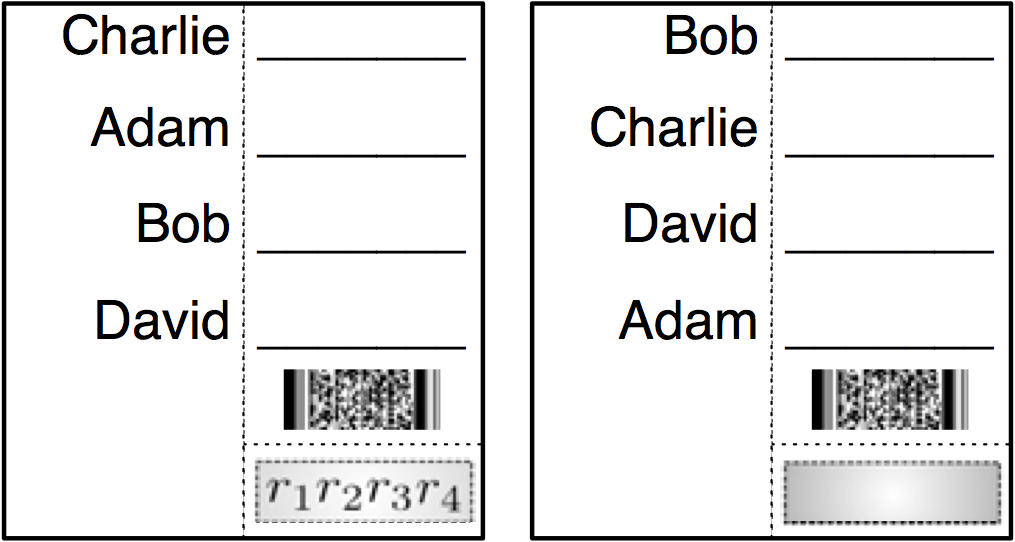
\includegraphics[width=0.5\linewidth]{ls/scratch_and_vote_ballot.png}}
  \caption{Scratch \& Vote biljet\cite{adida_rivest_scratch_and_vote}}
  \label{fig:ls:scratch_and_vote_ballot}
\end{figure}

\npar Voor de encryptie wordt gebruik gemaakt van het Paillier public key cryptosystem. Dit systeem heeft een additief homomorfisme door het vermenigvuldigen van de cijferteksten. Het tellen van de stemmen bij een verkiezing met meerdere kandidaten zou echter niet mogelijk zijn zonder gebruik te maken van een multi-counter. Het aantal beschikbare bits voor de leesbare tekst wordt onderverdeeld in verschillende tellers. Hierbij worden voldoende bits beschikbaar gemaakt voor elke teller zodat ze niet in elkaar kunnen overlopen.

\npar Het systeem maakt daarnaast gebruik van zero-knowledge bewijzen. Deze worden gebruikt om aan te tonen dat een set cijferteksten $c_1, c_2, \ldots, c_l$ de encryptie is van de permutatie van $m_1, m_2, \ldots, m_k$ (ervan uitgaande dat geen twee subsets van ${m_i}$ dezelfde som hebben). De verschillende ${m_i}$ zijn de tellers voor de kandidaten.

\npar Daarnaast worden ook bewijzen opgesteld die aantonen dat de biljetten zelf correct zijn. Omdat deze bewijzen te lang zijn om op de biljetten te printen, worden ze voor de start van de verkiezing ge\"upload naar het bulletin board. Ze worden tijdens het tellen van de stemmen gebruikt om te verzekeren dat elk biljet maar \'e\'en stem uitbrengt per verkiezing. Om de kiezer te garanderen dat zijn biljet tijdens het tellen niet ongeldig verklaard zal worden, wordt ook een offici\"ele lijst van alle geldige biljetten voorzien. De kiezer kan dan eenvoudig nagaan of zijn biljet hierop voorkomt.

\begin{figure}[H]
  \center{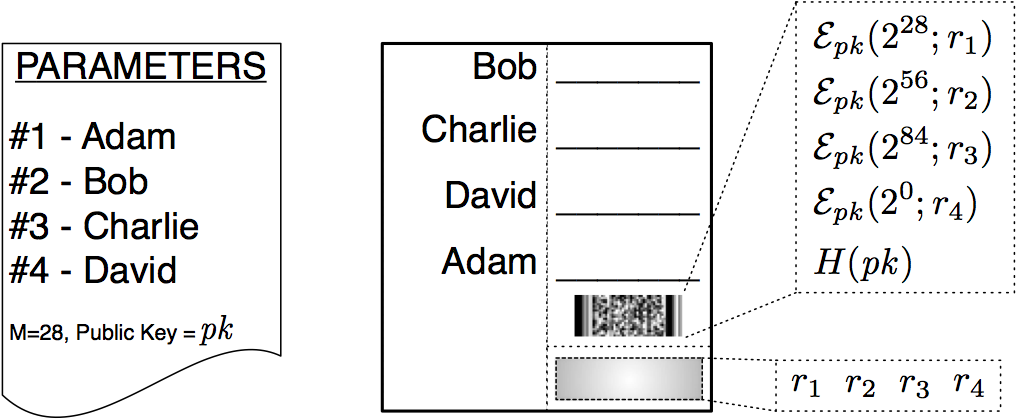
\includegraphics[width=0.5\linewidth]{ls/scratch_and_vote_encryption.png}}
  \caption{Scratch \& Vote encryptie\cite{adida_rivest_scratch_and_vote}}
  \label{fig:ls:scratch_and_vote_encryption}
\end{figure}

\npar De 2D barcode op elk biljet encodeert de willekeurige volgorde van de cijferteksten voor de verschillende kandidaten samen met een hash van de publieke sleutel (\ref{fig:ls:scratch_and_vote_encryption}). De startwaarde van de teller van elke kandidaat wordt samen met een willekeurige waarde ge\"encrypteerd. Zo heeft elk biljet een unieke cijfertekst voor elke kandidaat. Deze willekeurige waarden worden verborgen door de kraslaag. De startwaarden van de tellers vormen samen met de publieke sleutel de gepubliceerde parameters. Samen met de willekeurige waarden kunnen ze dus gebruikt worden om de volgorde van de kandidaten op het biljet te achterhalen. Daarom is het belangrijk dat dit stukje van het biljet vernietigd wordt.

\npar Deze informatie wordt toch op de biljetten geprint omdat ze nodig zijn voor een audit. Dit wordt gedaan door de kiezer twee biljetten te laten kiezen. Door de kraslaag weg te halen, worden de willekeurige waarden zichtbaar en kan nagegaan worden of het biljet correct is. Door het verwijderen van de kraslaag wordt het biljet ongeldig, wat de reden is dat de kiezer twee biljetten moet nemen. Op deze manier wordt de helft van de biljetten getest en dus is de kans groot dat foutieve biljetten gedetecteerd worden.

\npar Zowel naar de kiezer als de bijzitters is dit systeem zeer gebruiksvriendelijk. Het standaard stembiljet is slechts licht gewijzigd en de kiezer zou er dus vertrouwd mee moeten zijn. Ook de stemprocedure is niet radicaal gewijzigd. Aangezien de telprocedure ook geautomatiseerd is, kan deze methode ook voor grote verkiezingen gebruikt worden.

\section{Conclusie}
\label{sec:ls:conclusie}

Bij open counting (\ref{sec:ls:open_counting}) wordt een transparante manier van tellen gebruikt om het vertrouwen van de kiezer in het resultaat te vergroten. In tegenstelling tot de andere systemen kan hier door de kiezer wel niet nagegaan worden of zijn stem meegeteld is. Voter-verifiability wordt daar bekomen door gebruik te maken van een ander type biljet samen met een aangepaste stemprocedure.

\npar Deze aanpassingen maken het stemmen voor de kiezer ingewikkelder. In tegenstelling tot bij een klassiek biljet, moeten nu verschillende regels gevolgd worden om het biljet correct in te vullen. De stemprocedures zijn vaak ook ingewikkelder dan voordien, met nieuwe regels voor zowel de kiezers als de bijzitters.

\npar Door cryptografische technieken te gebruiken, kan de gebruiksvriendelijkheid van papieren end-to-end verifiable systemen sterk verbeterd worden. Een nadeel is hier dan weer dat de meeste mensen nog steeds zullen moeten vertrouwen op het oordeel van een expert over de correctheid van het systeem.

\npar Papieren voter-verifiable systemen hebben dus enkele grote nadelen die hun praktisch nut sterk beperken. Ze zijn vaak zeer complex en niet bruikbaar voor grote verkiezingen. Cryptografische technieken lossen deze problemen wel deels op, maar worden dan weer moeilijker vertrouwd door de kiezer.

  
  % 
% Helios
% @author Pieter Maene <pieter.maene@student.kuleuven.be>
%

\chapter{Helios}
\label{chap:helios}

Het Helios verkiezingssysteem is een open-source project dat geleid wordt door Ben Adida.\cite{adida_helios} Het laat toe om online voter-verifiable verkiezingen te organiseren. Zoals vermeld in \ref{sec:ls:online_stemmen} kunnen online verkiezingen alleen gebruikt worden in een context waar dwang geen grote bedreiging vormt. Dit systeem werd vorig jaar door Robbert Coeckelbergh uitgebreid met threshold encryptie en gerangschikte verkiezingen.\cite{coeckelbergh_toepassing_en_uitbreiding_van_het_helios_online_verkiezingssysteem} 

\npar In dit hoofdstuk worden de belangrijkste cryptografische technieken uitgelegd die Helios gebruikt (\ref{sec:helios:cryptografische_technieken}). Daarna wordt de functionaliteit van de publieke delen van Helios besproken: het stemhokje (\ref{sec:helios:stemhokje}), het ballot tracking center (\ref{sec:helios:ballot_tracking_center}) en de controleapplicatie (\ref{sec:helios:controleapplicatie}).

\section{Cryptografische technieken}
\label{sec:helios:cryptografische_technieken}

Op het vlak van cryptografische technieken leunt Helios het dichtste aan bij Scratch \& Vote (\ref{sec:ls:scratch_and_vote}). Ook in Helios worden de stemmen ge\"encrypteerd. Na het aflopen van de stemming worden alle biljetten homomorf opgeteld. Tot slot wordt het resultaat gedecrypteerd. Alle ge\"encrypteerde stemmen worden ook online gepubliceerd, zodat iedereen kan verifi\"eren of het resultaat correct is.

\npar Het belangrijkste verschil is dat ElGamal gebruikt wordt in plaats van Paillier voor de homomorfe encryptie van de stemmen (\ref{sec:helios:elgamal} en \ref{sec:helios:homomorfe_encryptie}). Tot slot wordt de methode besproken waarop de sleutel verdeeld wordt tussen de trustees (\ref{sec:helios:threshold_encryptie}).

\subsection{ElGamal~\cite{elgamal_elgamal}}
\label{sec:helios:elgamal}

Het ElGamal \textit{cryptosystem} is een asymmetrisch schema dat gebaseerd is op het Diffie-Hellman protocol. Dit betekent dat een sleutelpaar met zowel een geheime als publieke sleutel nodig is. De publieke sleutel wordt gebruikt om de klaartekst te encrypteren. De decryptie kan alleen uitgevoerd worden met de geheime sleutel.

\npar Er wordt gewerkt in de groep $\mathbb{Z}_p$ waar $g$ de generator is. Hierbij is $p$ een veilig priemgetal dat deelbaar is door het priemgetal $q$. De geheime sleutel $sk$ wordt willekeurig gekozen binnen $\mathbb{Z}_{p-1}$. De publieke sleutel is dan ${pk} = g^{sk} \mod{p}$. De cijfertekst van een ElGamal encryptie bestaat uit twee delen: $c_1$ (\ref{eq:helios:elgamal_c1}) en $c_2$ (\ref{eq:helios:elgamal_c2}). In deze vergelijkingen is $m$ de klaartekst en $r$ opnieuw een willekeurig getal binnen $\mathbb{Z}_{p-1}$. $c_1$ en $r$ hebben respectievelijk de functie van tijdelijke publieke en private sleutel.\cite{preneel_cryptography_and_network_security}

\begin{align}
  \label{eq:helios:elgamal_c1} 
  c_1 & = g^r \mod{p} \\
  \label{eq:helios:elgamal_c2}
  c_2 & = m \cdot {pk}^r \mod{p}
\end{align}

\npar De cijfertekst kan dan gedecrypteerd worden volgens \ref{eq:helios:elgamal_m}.

\begin{equation}
  \label{eq:helios:elgamal_m}
  m = \frac{c_2}{c_1^{sk}} \mod{p}
\end{equation}

\subsection{Homomorfe encryptie}
\label{sec:helios:homomorfe_encryptie}

Bij homomorfe encryptie kan een specifieke operatie met de cijfertekst uitgevoerd worden. De resulterende cijfertekst is de encryptie van een bepaalde bewerking op de klaarteksten.\cite{wiki:homomorphic_encryption} Zo is het Paillier cryptosystem dat gebruikt wordt in Scratch \& Vote (\ref{sec:ls:scratch_and_vote}) homomorf onder $(\times, +)$. Dit betekent dat een vermenigvuldiging van de cijferteksten resulteert in een optelling van de klaarteksten.

\npar Het homomorfisme $(\times, +)$ kan in een verkiezingssysteem gebruikt worden om effici\"ent de stemmen op te tellen. De berekening van het resultaat kan immers gebeuren aan de hand van de cijferteksten. Er moet nu alleen een decryptie gebeuren om het uiteindelijke resultaat vrij te geven.

\npar Aan de hand van \ref{eq:helios:elgamal_c2} kan gezien worden dat ElGamal standaard homomorf is onder $(\times, \times)$. Zoals hiervoor besproken, is voor een verkiezingssysteem echter het homomorfisme $(\times, +)$ nodig. Dit kan gerealiseerd worden door de klaartekst ook in de exponent te plaatsen (\ref{eq:helios:elgamal_c2_homomorphic}).

\begin{equation}
  \label{eq:helios:elgamal_c2_homomorphic}
  c_2 = g^m \cdot {pk}^r \mod{p}
\end{equation}

\ref{eq:helios:elgamal_homomorphic} geeft het homomorfisme dat zo bekomen wordt.

\begin{equation}
  \label{eq:helios:elgamal_homomorphic}
  \begin{array}{lcl}
    \mathcal{E}(m_1) \cdot \mathcal{E}(m_2) &=& (g^{r_1}, g^{m_1} \cdot {pk}^{r_1}) \cdot (g^{r_2}, g^{m_2} \cdot {pk}^{r_2}) \\
      &=& (g^{r_1 + r_2}, g^{m_1 + m_2} \cdot {pk}^{r_1 + r_2}) \\
      &=& \mathcal{E}(m_1 + m_2)
  \end{array}
\end{equation}

\npar Omwille van het discreet logaritme probleem is het terugvinden van $m$ echter niet meer zo vanzelfsprekend.\cite{menezes_vanstone_oorschot_handbook_of_applied_cryptography} Dit kan alleen gedaan worden door $g^m \mod{p}$ te berekenen voor elke $m$ en vervolgens te zoeken welke hetzelfde is als de klaartekst van de decryptie.

\npar Scratch \& Vote (\ref{sec:ls:scratch_and_vote}) gebruikt multi-counters voor een stemming met meerdere kandidaten. Helios daarentegen encrypteert ieder mogelijk antwoord op een vraag afzonderlijk. Wanneer het antwoord gekozen wordt, is $m = 1$; anders wordt $m = 0$ gesteld.

\subsection{Threshold encryptie}
\label{sec:helios:threshold_encryptie}

Oorspronkelijk kon de publieke sleutel voor de verkiezing alleen berekend worden als het product van de afzonderlijke publieke sleutels van de \textit{trustees} (\ref{eq:helios:elgamal_c2_homomorphic_trustees}). Voor de decryptie moet iedere trustee zijn factor uit de noemer van \ref{eq:helios:elgamal_m_homomorphic_trustees} berekenen. Deze factoren worden in Helios de decryptiefactoren genoemd.

\begin{equation}
  \label{eq:helios:elgamal_c2_homomorphic_trustees}
  PK = \prod_{i=1}^n{{pk}_i} \mod{p}
\end{equation}

\begin{equation}
  \label{eq:helios:elgamal_m_homomorphic_trustees}
  g^m = \frac{c_2}{\prod_{i=1}^n{c_1^{{sk}_i}}} = \frac{c_2}{\prod_{i=1}^n{{df}_i}} \mod{p}
\end{equation}

\npar Een groot probleem hierbij is dat wanneer \'e\'en trustee zijn geheime sleutel verliest, het resultaat niet meer gedecrypteerd kan worden. Daarom werd threshold encryptie toegevoegd door Robbert Coeckelbergh.\cite{coeckelbergh_toepassing_en_uitbreiding_van_het_helios_online_verkiezingssysteem} Er kan nu een threshold schema gedefinieerd worden zodat slechts $k$ van de $n$ trustees hun decryptiefactor moeten berekenen.

\subsubsection{Secret Sharing}

De methode die ge\"implementeerd werd, is gebaseerd op Shamir's secret sharing.\cite{shamir_how_to_share_a_secret} Iedere trustee genereert eerst een veelterm van graad $k - 1$. Vervolgens stuurt hij elke trustee (ook zichzelf) een zogeheten \textit{share} van deze veelterm. Deze share is de waarde van de veelterm voor een punt $x$. Deze $x$-co\"ordinaat moet door iedereen gekend zijn, omdat het vereist is dat de shares die een trustee ontvangt van de anderen voor dezelfde waarde werden aangemaakt. Daarom wordt hiervoor binnen Helios het database ID van de trustee gebruikt. Dit is een uniek natuurlijk getal dat wordt opgehoogd telkens een nieuwe trustee aangemaakt wordt. Door \textit{zero-knowledge} bewijzen op te stellen, wordt heel dit proces verifiable. Hier wordt echter niet verder op ingegaan.

\npar Vervolgens moet de trustee de $n$ shares die hij zo ontvangt, optellen. Zo bekomt hij de $y$-co\"ordinaat die hoort bij zijn ID op een nieuwe veelterm, die de som is van de $n$ veeltermen die door de trustees gegenereerd werden. Deze waarde kan hij nu gebruiken als zijn geheime sleutel ${sk}$. Omdat ElGamal gebruikt wordt als encryptieschema, wordt zijn publieke sleutel ${pk} = g^{sk} \mod{p}$.

\npar Als geheime sleutel voor de verkiezing wordt nu de waarde voor $x = 0$ op de gemeenschappelijke veelterm genomen. Deze veelterm kan door Lagrange-interpolatie gereconstrueerd worden uit $k$ punten. Hiervoor worden de eerste $k$ trustees gebruikt (dat zijn deze met het laagste ID). Omdat alleen de publieke sleutels van de trustees beschikbaar zijn, wordt echter onmiddellijk de publieke sleutel voor de verkiezing berekend (\ref{eq:helios:threshold_encryption_public_key}).

\begin{align}
  \label{eq:helios:threshold_encryption_lagrange}
  \lambda_i(x) & = \prod_{j=1, j\not=i}^k{\frac{x - x_j}{x_i - x_j}} \\
  \label{eq:helios:threshold_encryption_polynomial}
  V(x) & = \sum_{i=1}^k{{sk}_i\lambda_i(x)}
\end{align}

\begin{align}
  \label{eq:helios:threshold_encryption_secret_key}
  SK & = V(0) = \sum_{i=1}^k{{sk}_i\lambda_i(0)} \\
  \label{eq:helios:threshold_encryption_public_key}
  PK & = g^{X} = \prod_{i=1}^k{{pk}_i^{\lambda_i(0)}} \mod{p}
\end{align}

\npar Om het resultaat te decrypteren, moet de geheime sleutel voor de verkiezing gebruikt worden (\ref{eq:helios:threshold_encryption_secret_key}). Het grote voordeel van threshold encryptie is dat het hier niet belangrijk is van welke $k$ trustees de decryptiefactoren en bijhorende Lagrange-interpolatie gebruikt worden.

\begin{equation}
  \label{eq:helios:threshold_encryption_m}
  g^m = \frac{c_2}{\prod_{i=1}^k{c_1^{{sk}_i\lambda_i(0)}}} = \frac{c_2}{\prod_{i=1}^k{{df}_i^{\lambda_i(0)}}} \mod{p}
\end{equation}

\subsubsection{Communicatiesleutels}
\label{sec:helios:communicatiesleutels}

Voordat iedere trustee zijn gegenereerde shares doorstuurt naar de andere trustees, worden deze ge\"encrypteerd en getekend. Hiervoor worden respectievelijk de publieke sleutel voor encryptie en de publieke sleutel voor tekenen van de andere trustee gebruikt. Dit geeft aanleiding tot twee nieuwe sleutelparen die de communicatiesleutels genoemd worden.

\section{Toepassing in Helios}

De cryptografische technieken van \ref{sec:helios:cryptografische_technieken} worden in Helios gebruikt om de stemmen te encrypteren (\ref{sec:helios:stemhokje}). Het Ballot Tracking Center is het publieke bulletin board uit Scratch \& Vote waarop alle kiezers en hun stem gepubliceerd worden (\ref{sec:helios:ballot_tracking_center}). De controleapplicatie (\ref{sec:helios:controleapplicatie}) kan gebruikt worden door de kiezer om na te gaan of het resultaat correct is.

\subsection{Stemhokje}
\label{sec:helios:stemhokje}

Het stemhokje staat volledig los van de rest van het systeem. Het is een applicatie die de kiezer kan gebruiken om zijn stem uit te brengen. Nadat hij zijn keuze gemaakt heeft, wordt deze ge\"encrypteerd met de publieke sleutel voor de verkiezing. Zoals besproken in \ref{sec:helios:cryptografische_technieken}, zal de cijfertekst bestaan uit twee delen (\ref{eq:helios:elgamal_c1} en \ref{eq:helios:elgamal_c2_homomorphic}). Wanneer threshold encryptie aanstaat, wordt de publieke sleutel zoals gedefinieerd door \ref{eq:helios:threshold_encryption_public_key} gebruikt; anders is het deze van \ref{eq:helios:elgamal_c2_homomorphic_trustees}. Daarnaast worden ook zero-knowledge bewijzen opgesteld voor de stem, maar hier wordt niet dieper op ingegaan.

\npar Het encryptieproces is in JavaScript ge\"implementeerd en vindt dus volledig plaats in de browser van de kiezer. Zijn stem zal dan ook nooit onge\"encrypteerd op de server toekomen. Alle informatie over de verkiezing kan eenvoudig opgevraagd worden. De kiezer zou dus ook zijn eigen software kunnen gebruiken om zijn stem te encrypteren.

\npar Aan elke ge\"encrypteerde stem wordt een \textit{smart ballot tracker} toegekend. Dit is een fingerprint die de stem identificeert (\ref{sec:sf:fingerprints}). Aan de hand daarvan kan de kiezer zijn stem volgen doorheen het systeem en kan hij verifi\"eren of ze niet aangepast is.

\subsection{Ballot Tracking Center}
\label{sec:helios:ballot_tracking_center}

Net zoals bij Scratch \& Vote (\ref{sec:ls:scratch_and_vote}) worden de uitgebrachte stemmen gepubliceerd. In het ballot tracking center kan een lijst met alle kiezers teruggevonden worden. Bij een publieke verkiezing kan iedereen deze opvragen, bij een private alleen de geregistreerde kiezers. Standaard staan hier gewoon de namen van de kiezers, maar de beheerder kan ervoor kiezen om aliassen te gebruiken in de plaats.

\npar Van zodra een kiezer zijn stem uitgebracht heeft, kan deze door iedereen bekeken worden (\ref{fig:helios:cast_vote}). Dit is nodig omdat zo het resultaat van de verkiezing gecontroleerd kan worden (\ref{sec:helios:controleapplicatie}). Al deze informatie kan ook opgevraagd worden als JSON, zodat de applicatie ze eenvoudiger kan verwerken. Een derde partij zou deze functionaliteit dus ook zelf kunnen implementeren.

\begin{figure}
  \center{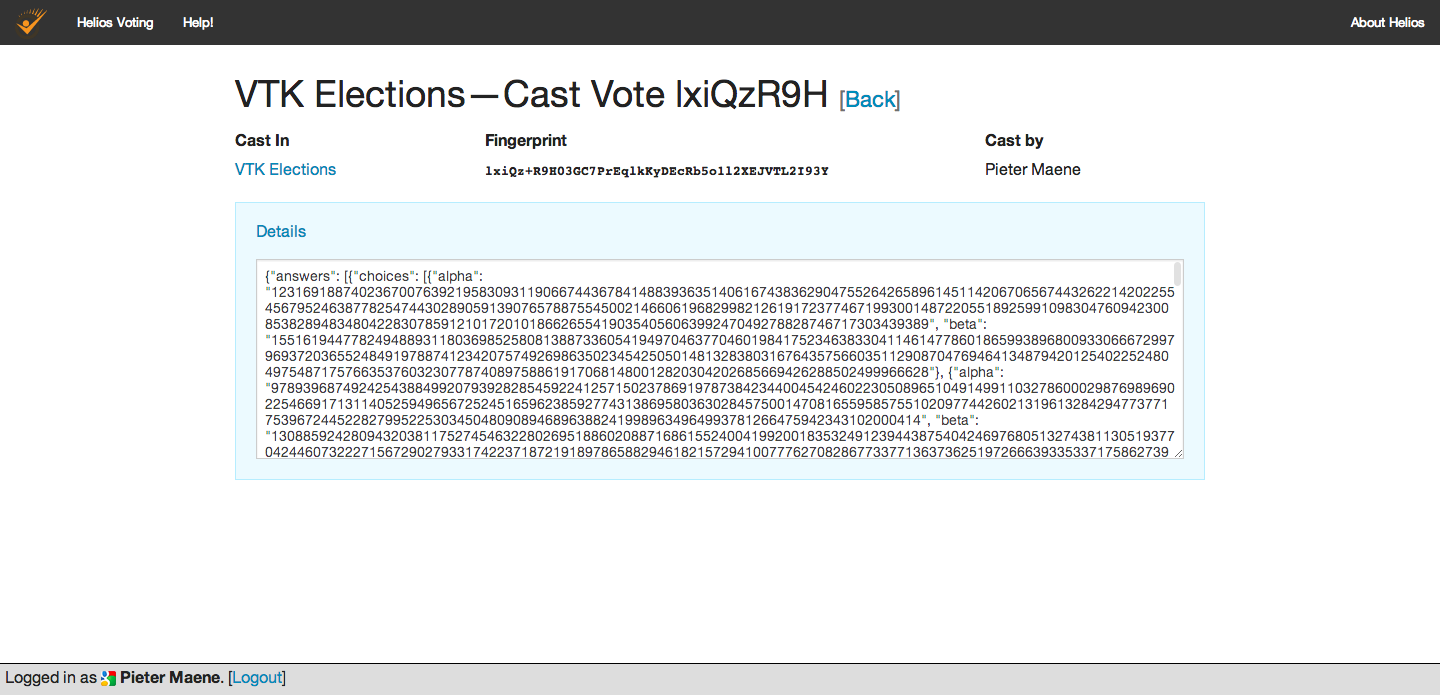
\includegraphics[width=0.9\linewidth]{helios/cast_vote.png}}
  \caption{Uitgebrachte stem}
  \label{fig:helios:cast_vote}
\end{figure}

\subsection{Controleapplicatie}
\label{sec:helios:controleapplicatie}

Net zoals het stemhokje is de controleapplicatie onafhankelijk en draait ze lokaal in de browser van de gebruiker. Ze kan gebruikt worden om het resultaat van de verkiezing te controleren. Alle ruwe data wordt gedownload van de server, waarna de nodige berekeningen lokaal worden uitgevoerd.

  % 
% Procedure
% @author Pieter Maene <pieter.maene@student.kuleuven.be>
%

\chapter{Verkiezingsprocedure in Helios}
\label{chap:procedure}

Dit hoofdstuk geeft de procedure die in de aangepaste versie van Helios gevolgd moet worden om een verkiezing op te zetten. In \ref{sec:proc:voorbereiding} wordt bekeken welke informatie gekend moet zijn voordat het aanmaken van de verkiezing aangevat wordt. De procedure zelf wordt in \ref{sec:proc:helios} beschreven.

\section{Voorbereiding}
\label{sec:proc:voorbereiding}

\subsection{Trustees}

De trustees zijn de personen die verantwoordelijk zullen zijn voor het decrypteren van het resultaat. Aangezien zij een belangrijke rol spelen in het verkiezingsproces, is het belangrijk dat de beheerder vooraf vastlegt wie dit zal doen. Helios heeft ondersteuning voor threshold encryptie (\ref{sec:helios:threshold_encryptie}). Er moet dus ook nagedacht worden over het threshold schema: hoeveel trustees nodig zullen zijn om het resultaat van de verkiezing te decrypteren. Om een trustee aan te maken, moeten zijn naam en een geldig e-mailadres opgegeven worden.

\subsection{Vragen}
\label{sec:proc:voorbereiding:vragen}

Het belangrijkste van de verkiezing zijn uiteraard de vragen die de kiezers zullen moeten beantwoorden. Bij elke vraag kan in Helios aangegeven worden hoeveel antwoorden elke kiezer kan aanduiden, dus de beheerder moet ook dit op voorhand bepalen. Het resultaat kan ofwel absoluut ofwel relatief weergegeven worden. In het eerste geval zal bij elke optie het aantal stemmen voor deze optie getoond worden, in het tweede alleen de relatieve plaatsen van de opties onderling.

\subsection{Kiezers}
\label{sec:proc:voorbereiding:kiezers}

Een verkiezing in Helios kan door de beheerder opengesteld worden voor iedereen of voor specifieke kiezers. Bij een gesloten verkiezing moet op voorhand een lijst van geldige kiezers opgesteld worden.

\npar Deze kiezers kunnen in Helios ge\"importeerd worden door een CSV-bestand aan te maken. Helios heeft van elke kiezer de volledige naam en een uniek ID nodig. Het e-mailadres van de kiezer kan opgegeven worden, maar dit is niet vereist. Er kan ook aangegeven worden welk authenticatiesysteem (bv. Google of Shibboleth) gebruikt wordt door de kiezer. Wanneer dit laatste veld leeg is, zal een gegenereerd wachtwoord naar hem opgestuurd worden.

\section{Helios setup}
\label{sec:proc:helios}

\subsection{Aanmaken van de verkiezing}

De eerste stap is het aanmaken van de verkiezing. Hier moet de basisinformatie van de verkiezing opgegeven worden zoals de naam en het type verkiezing. Ofwel kan er een verkiezing aangemaakt worden, ofwel een referendum. Voor beide types is de procedure echter identiek.

\begin{figure}
  \center{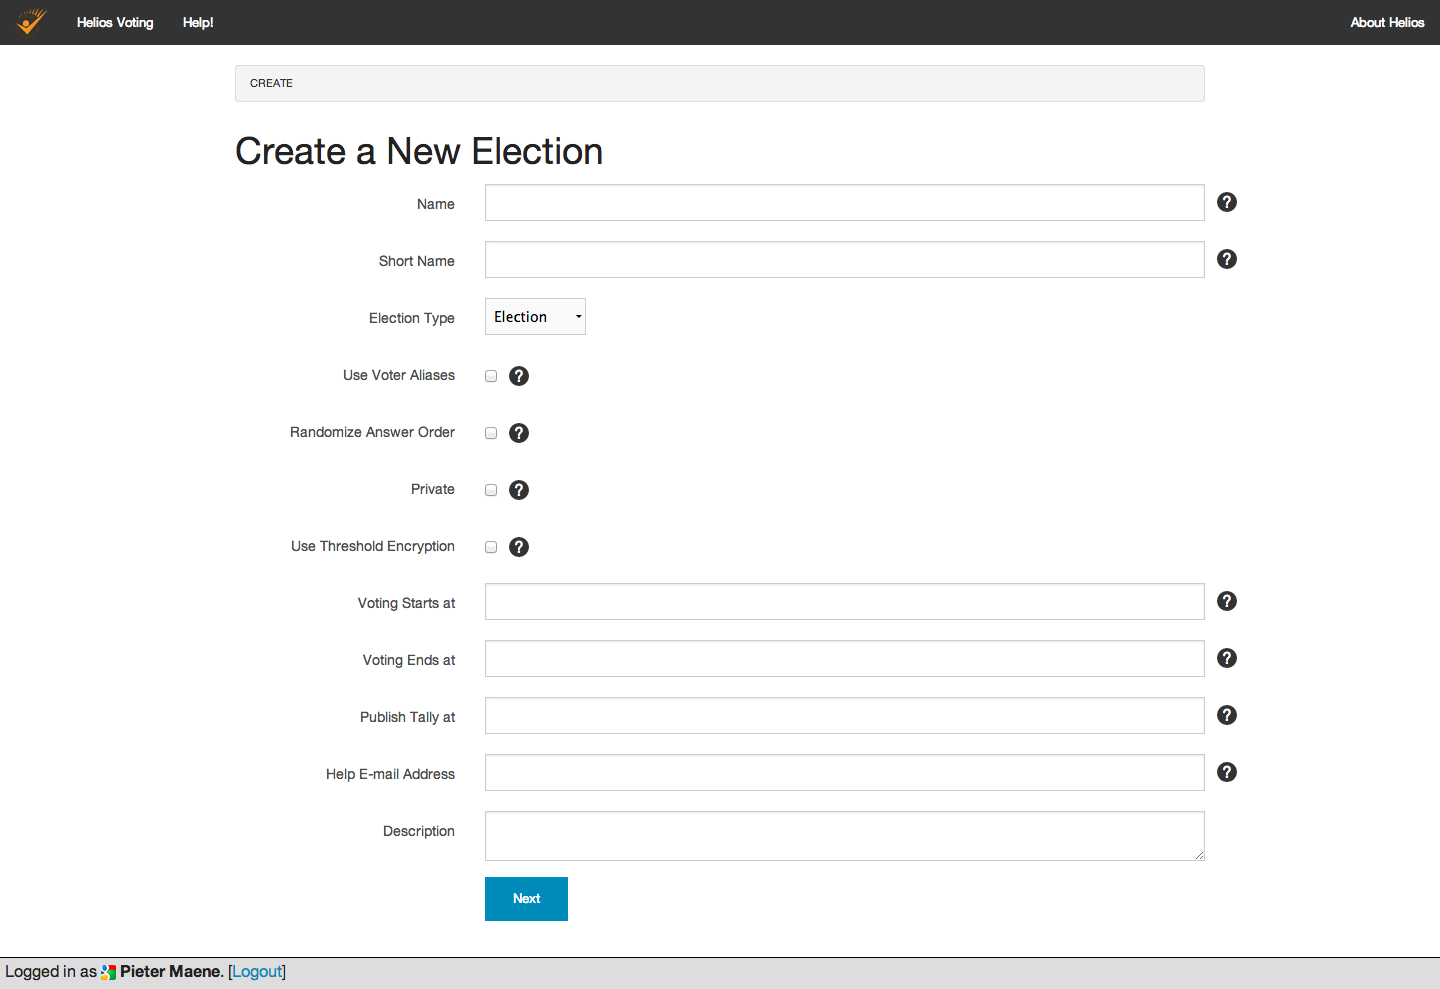
\includegraphics[width=0.9\linewidth]{proc/elections_new.png}}
  \caption{Aanmaken van de verkiezing}
  \label{fig:proc:elections_new}
\end{figure}

\npar Vervolgens kunnen een aantal belangrijke functies aan- of uitgezet worden. Wanneer aliassen gebruikt worden, dan worden de namen van de kiezers verborgen in het publieke ballot tracking center (\ref{sec:helios:ballot_tracking_center}). Het is ook mogelijk om de antwoorden in een random volgorde op het biljet te laten zetten. Een geheime verkiezing kan alleen bekeken worden door de geregistreerde kiezers. Deze moet dus gebruikt worden wanneer kieslijsten beschikbaar zijn. Hier moet ook aangegeven worden of threshold encryptie  (\ref{sec:helios:threshold_encryptie}) toegepast zal worden. Het is aangeraden dit aan te zetten, aangezien deze techniek resulteert in een robuuster decryptieproces.

\npar Tot slot is het mogelijk om aan te geven wanneer de verkiezing moet starten en sluiten. Wanneer het resultaat niet onmiddellijk na het aflopen van de verkiezing gepubliceerd mag worden, kan hiervoor een alternatief tijdstip opgegeven worden.

\subsection{Trustees}
\label{sec:proc:trustees}

Eens de nieuwe verkiezing aangemaakt is, moeten de trustees toegevoegd worden. Deze stap is eerst gezet in de procedure omdat hij veruit de meeste tijd in beslag neemt. De beheerder van de verkiezing moet eerst alle trustees aanmaken. De trustee krijgt dan meteen een link toegestuurd via e-mail naar zijn trustee dashboard (\ref{sec:ui:trustee_dashboard}) waar hij al zijn acties zal moeten uitvoeren.

\begin{figure}
  \center{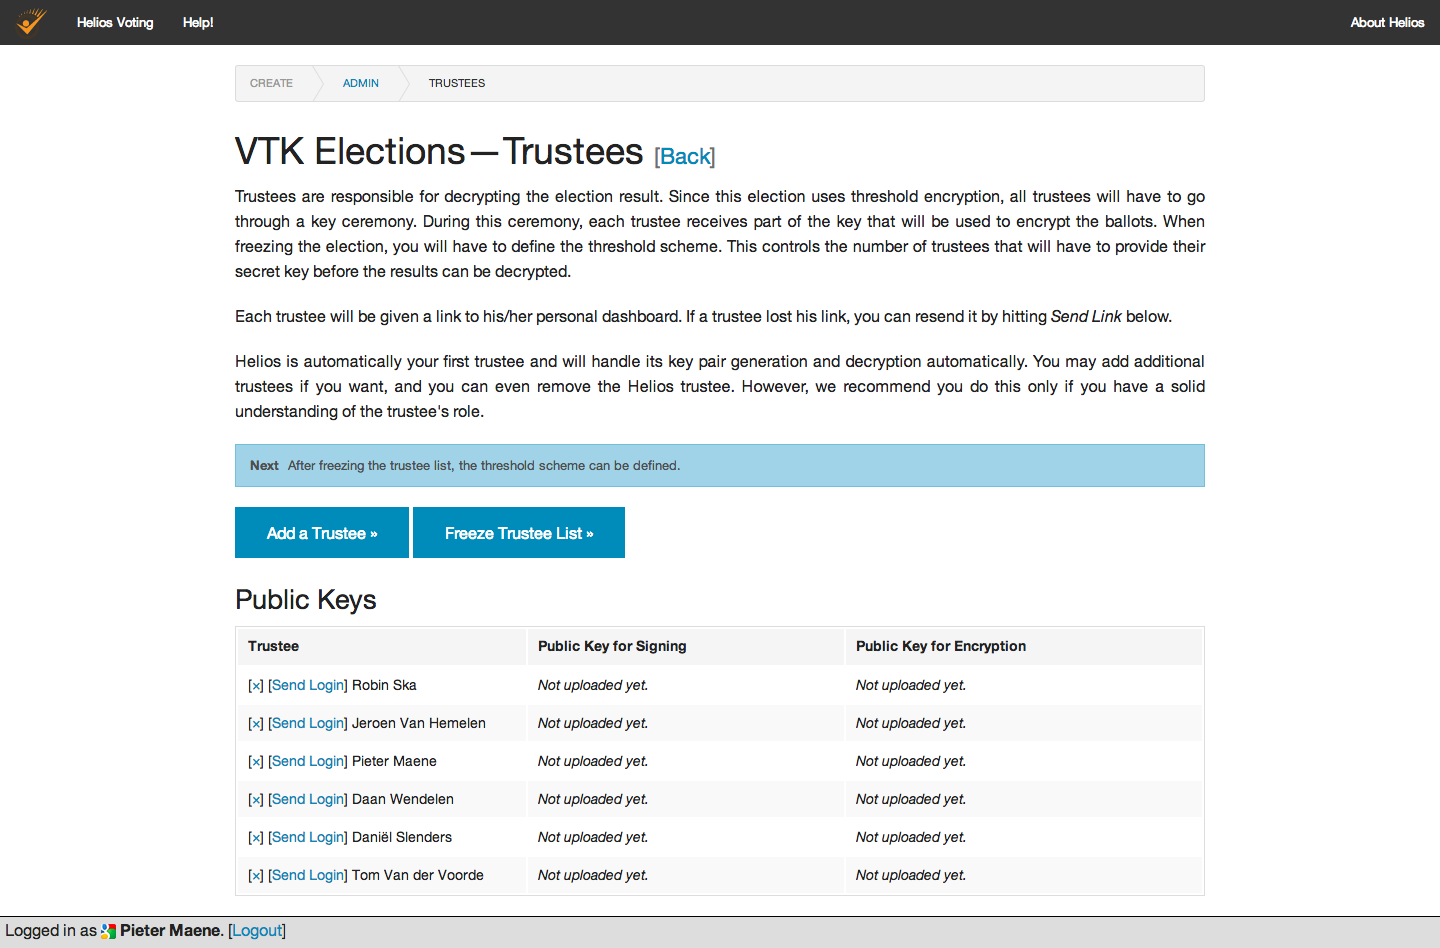
\includegraphics[width=0.9\linewidth]{proc/trustees_view.png}}
  \caption{Trustees}
  \label{fig:proc:trustees_view}
\end{figure}

\subsubsection{Verkiezing zonder threshold encryptie}

Wanneer geen threshold encryptie gebruikt wordt, is dit proces eenvoudig. Van zodra een trustee aangemaakt is, kan hij het sleutelpaar genereren dat gebruikt zal worden als deel van de sleutel voor de verkiezing. Alle trustees moeten dit gedaan hebben voordat de beheerder de verkiezing kan bevriezen en openstellen voor de kiezers. Hij kan ondertussen echter wel verdergaan met de procedure.

\subsubsection{Verkiezing met threshold encryptie}

\npar Wanneer alle trustees aangemaakt zijn, kan deze lijst bevroren worden. Op dit moment moet ook het threshold schema ingegeven worden. Eens dit gebeurd is, begint voor de trustees de sleutelceremonie. Deze bestaat uit drie stappen.

\begin{figure}
  \center{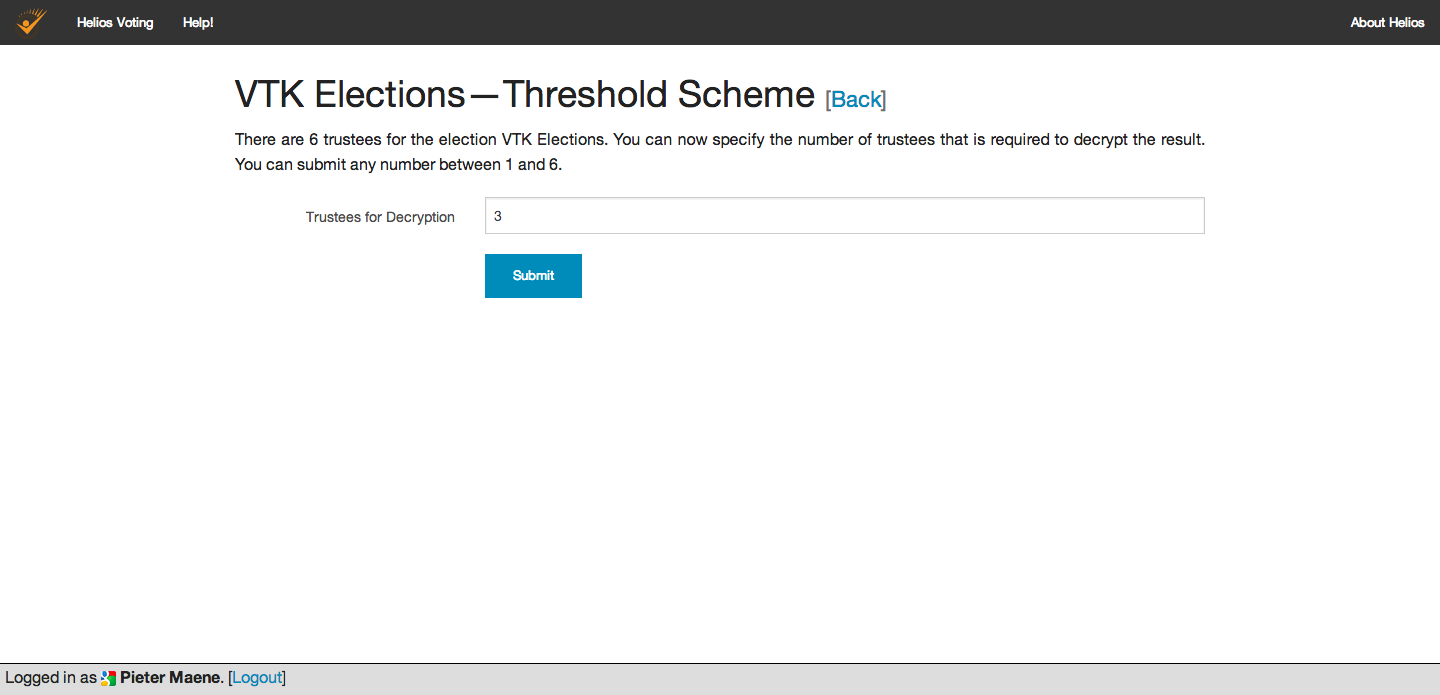
\includegraphics[width=0.9\linewidth]{proc/trustees_freeze.png}}
  \caption{Threshold schema}
  \label{fig:proc:trustees_freeze}
\end{figure}

\begin{enumerate}
  \item De trustees moeten eerst de twee sleutelparen genereren die gebruikt zullen worden om hun onderlinge communicatie te beveiligen. Pas wanneer alle trustees deze stap uitgevoerd hebben, kan verdergegaan worden.
  \item Elke trustee maakt vervolgens zijn shares aan en encrypteert deze voor de andere trustees. Hier moet opnieuw gewacht worden totdat alle trustees deze stap voltooid hebben.
  \item De trustees kunnen nu de shares die ze van de andere gekregen hebben decrypteren en optellen. Zo bekomen ze het sleutelpaar dat later gebruikt zal kunnen worden om de encryptiesleutel van de verkiezing de reconstrueren.
\end{enumerate}

Pas wanneer alle trustees de volledige sleutelceremonie doorlopen hebben, kan de verkiezing door de beheerder bevroren worden. Omdat de verschillende trustees dus vaak op elkaar moeten wachten, krijgen ze een e-mail elke keer de volgende stap uit de ceremonie aangevat kan worden.

\subsection{Vragen}

Terwijl de trustees bezig zijn met het uitvoeren van de sleutelceremonie, kan het stembiljet wel aangemaakt worden. Alle informatie die hiervoor nodig is, werd reeds voorbereid (\ref{sec:proc:voorbereiding:vragen}).

\begin{figure}
  \center{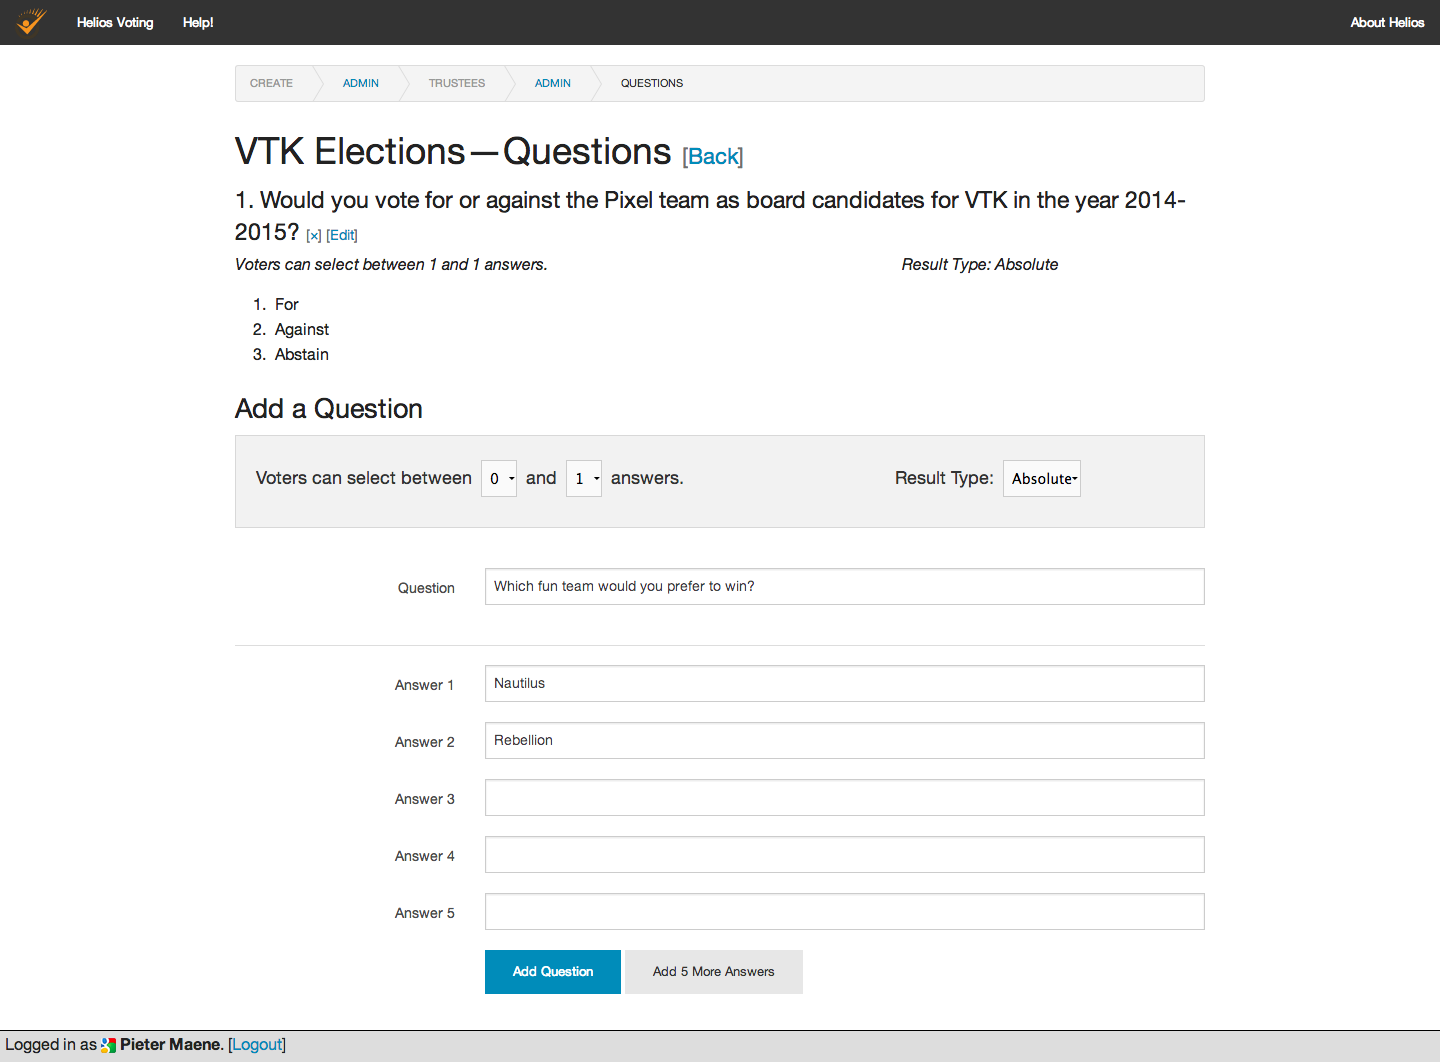
\includegraphics[width=0.9\linewidth]{proc/questions.png}}
  \caption{Vragen}
  \label{fig:proc:questions}
\end{figure}

\subsection{Kiezers}

Ook deze stap werd reeds volledig voorbereid (\ref{sec:proc:voorbereiding:vragen}). Hier kan de beheerder de CSV-bestanden uploaden, waarna het systeem ze verwerkt en alle kiezers toevoegt aan de verkiezing.

\begin{figure}
  \center{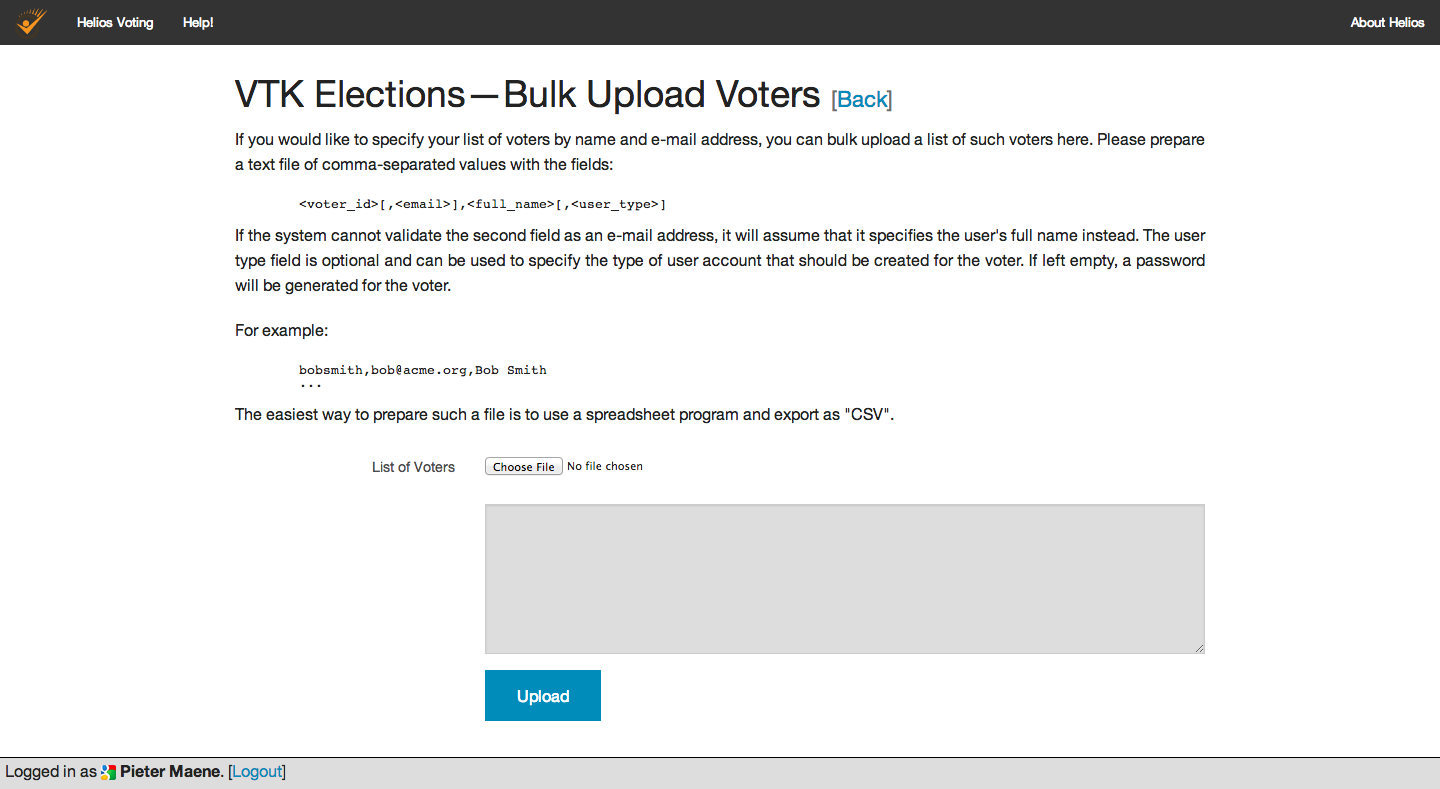
\includegraphics[width=0.9\linewidth]{proc/voters_upload.png}}
  \caption{Uploaden van kiezers}
  \label{fig:proc:voters_upload}
\end{figure}

\subsection{Bevriezen van het stembiljet}

Wanneer alle voorgaande informatie ingegeven is en de sleutelceremonie afgerond, kan het stembiljet bevroren worden. Wanneer er geen tijdsstip gegeven is waarop de verkiezing moet starten, kunnen de kiezers onmiddellijk beginnen stemmen. Wanneer geen einddatum opgegeven is, blijft ze open totdat de beheerder ze sluit.

\subsection{Telling}

De stemming kan steeds manueel afgesloten worden door het telproces te starten. De stemmen worden dan homomorf samengeteld in een geëncrypteerd resultaat (\ref{sec:helios:homomorfe_encryptie}). Vooraleer dit gedecrypteerd kan worden, moeten opnieuw gewacht worden op de trustees.

\npar Wanneer geen threshold encryptie gebruikt wordt, moeten alle trustees nu hun decryptiefactor berekenen en uploaden. Wordt dit wel gebruikt, dan moeten slechts $k$ van de $n$ trustees dit doen. Zodra alle nodige decryptiefactoren beschikaar zijn, kan de beheerder het resultaat vrijgeven. Indien geen publicatiedatum opgegeven werd, is het resultaat dan voor iedereen beschikbaar. Anders kan de beheerder het resultaat wel reeds bekijken, maar de andere kiezers pas op die datum.

\begin{figure}
  \center{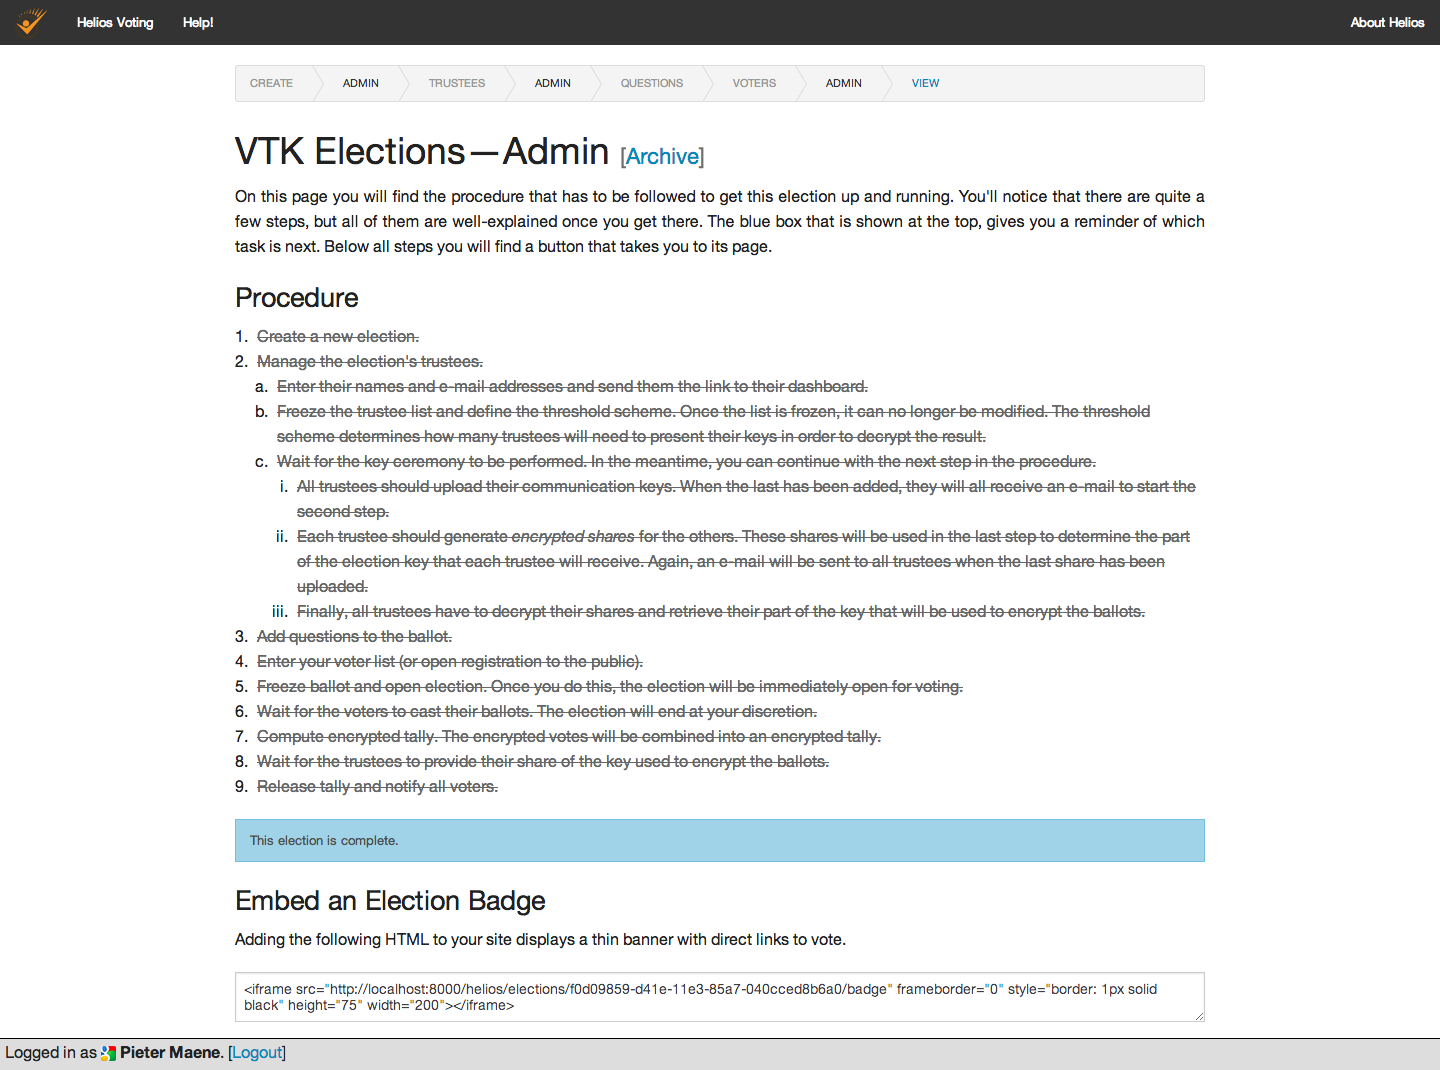
\includegraphics[width=0.9\linewidth]{proc/elections_admin.png}}
  \caption{Admin}
  \label{fig:proc:elections_admin}
\end{figure}

  % 
% Interface
% @author Pieter Maene <pieter.maene@student.kuleuven.be>
%

\chapter{Interface}
\label{chap:interface}

\section{Beheer}

\section{Trustee Dashboard}

\section{Stemhokje}

\section{Controleapplicatie}

  % 
% Kringverkiezing
% @author Pieter Maene <pieter.maene@student.kuleuven.be>
%

\chapter{Kringverkiezing}
\label{chap:kringverkiezing}

Het Helios verkiezingssysteem werd in de praktijk gebruikt tijdens de kringverkiezing van de Vlaamse Technische Kring. Dit is de faculteitskring van de studenten burgerlijk ingenieur aan de KU Leuven. Uit de kiesreglementen van VTK zelf en deze van LOKO volgen de vereisten waaraan het systeem moet voldoen (\ref{sec:kv:vereisten}). Om het systeem hiervoor te kunnen gebruiken, waren enkele aanpassingen nodig die overlopen worden in \ref{sec:kv:aanpassingen}. Gezien het cruciale karakter van een verkiezing, werd het systeem vervolgens uitgebreid getest (\ref{sec:kv:testen}). Tot slot wordt het verloop van de stemdag zelf besproken in \ref{sec:kv:stemdag}.

%TODO Remove Color

\section{Vereisten~\cite{loko_kiesreglement_verkiezingen}\cite{vtk_verkiezingsreglement}}
\label{sec:kv:vereisten}

%TODO Algemeen

\subsection{Trustees}

\textcolor{blue}{Het kiesreglement van LOKO schrijft voor dat over de verkiezingen gewaakt moet worden door een Neutraal Comit\'e. Dit wordt samengesteld door de huidige studentenvertegenwoordigers. Het Neutraal Comit\'e wordt bij VTK aangeduid met VKK. De huidige praeses is hier steeds de voorzitter van. Hij wordt geholpen door minstens vijf andere mensen uit het huidige praesidium die in een masteropleiding zitten en zelf geen kandidaat zijn in de verkiezing.}

\npar \textcolor{blue}{De voorzitter van VKK moet de verkiezing zelf kunnen beheren. Daarnaast moet het mogelijk zijn om alle leden van VKK aan te duiden als trustees van de verkiezing. Het mag ook niet mogelijk zijn dat \'e\'en trustee de decryptie van het resultaat kan blokkeren.}

\subsection{Vragen}

\textcolor{blue}{Er zijn twee verschillende types kiesploegen bij VTK. Enerzijds zijn er de serieuze ploegen die opkomen als praesidium voor het volgende jaar en anderzijds de lolploegen die niet als vertegenwoordigers verkiesbaar zijn. Beide verkiezingen moeten als aparte vragen op hetzelfde biljet gesteld kunnen worden.}

\textcolor{blue}{}


\subsection{Kiezers}

%TODO Kiezers
\textcolor{red}{}

\section{Aanpassingen}
\label{sec:kv:aanpassingen}

\subsection{Shibboleth}

Shibboleth is het authenticatie mechanisme dat gebruikt wordt voor de centrale login van de KU Leuven. Iedere gebruiker kan uniek ge\"identificeerd worden aan de hand van zijn studentennummer. Alle stemgerechtigde kiezers voor een kringverkiezing hebben een dergelijke account. Helios had hier echter nog geen ondersteuning voor. Gezien het modulaire ontwerp van het authenticatiesysteem, was dit relatief eenvoudig toe te voegen.

\npar De kieslijsten zelf werden opgemaakt door LOKO, de Leuvense studentenkoepel. Deze moesten wel nog omgezet worden naar een bestand dat uitgelezen kon worden door Helios. Het studentennummer werd hierbij gebruikt als het unieke ID voor elke kiezer. Een probleem was hier wel dat de e-mailadressen van de kiezers niet mee opgenomen waren in deze lijsten. Deze kunnen wel mee doorgegeven worden met het antwoord dat de server ontvangt nadat de student zich aangemeld heeft via de centrale login.

\subsection{Opkomst}

Bij VTK vertegenwoordigt het praesidium de studenten ook op onderwijsvlak. Om dit te kunnen doen, moet er volgens het reglement van LOKO een meerderheid behaald worden bij een opkomst van minstens 10\%.\cite{loko_kiesreglement_verkiezingen} De berekening van dit percentage werd dan ook toegevoegd zodat dit samen met de resultaten bekend gemaakt kon worden.

\subsection{Publicatie van het resultaat}

Helios publiceert het resultaat van de verkiezing standaard van zodra het bekend is. Het is echter traditie om deze pas om middernacht bekend te maken. Het systeem moest hier dus licht voor aangepast worden.

\section{Testen}
\label{sec:kv:testen}

Om er zeker van te zijn dat het systeem op de stemdag zelf goed zou functioneren, werd het na de installatie op de server getest. Hierbij werd niet alleen nagegaan of alles technisch in orde was, maar werd ook feedback gevraagd over de gebruiksvriendelijkheid. De testen van het beheer (\ref{sec:kv:beheer}) en het stemhokje (\ref{sec:kv:stemhokje}) werden uitgevoerd in de context van de vereisten voor VTK (\ref{sec:kv:vereisten}).

\subsection{Beheer}
\label{sec:kv:beheer}

Aangezien hier de meeste veranderingen gebeurd zijn (\ref{sec:ui:beheer}), moest zeker dit deel goed getest worden. Hiervoor werd een testverkiezing aangemaakt door de voorzitter van VKK, met de echte trustees en vragen. De echte kieslijsten werden vervangen door een lijst met de huidige praesidiumleden.

\npar De trustees voor de verkiezing zijn de zes leden van VKK. Als threshold schema (\ref{sec:helios:threshold_encryptie}) werd ervoor gekozen dat drie van hen nodig zijn om het resultaat te decrypteren. Tijdens deze test kwamen echter twee fouten naar boven. Ten eerste werd de Lagrange-interpolatie niet over het eindig veld berekend, maar met een rationale breuk. Wanneer slechts twee trustees gebruikt werden, was dit geen probleem omdat de noemer dan gelijk is aan \'e\'en. Dit kon eenvoudig opgelost worden door de teller en noemer voor het hele product apart te berekenen (\ref{eq:kv:modular_lagrange_numerator} en \ref{eq:kv:modular_lagrange_denominator}). Vervolgens wordt de teller vermenigvuldigd met de modulaire inverse van de noemer (\ref{eq:kv:modular_lagrange_result}).

\begin{align}
  \label{eq:kv:modular_lagrange_numerator} 
  N_i & = \prod_{j=1, j\not=i}^k{-x_j} \mod{q} \\
  \label{eq:kv:modular_lagrange_denominator}
  D_i & = \prod_{j=1, j\not=i}^k{(x_i - x_j)} \mod{q} \\
  \label{eq:kv:modular_lagrange_result}
  \lambda{_i}(0) & = N_i * (D_i^{-1} \mod{q}) \mod{q}
\end{align}

\npar Ten tweede werd de Helios trustee automatisch toegevoegd als trustee aan de verkiezing. Alle acties die een trustee moet uitvoeren, waren hiervoor geautomatiseerd. Na het uitvoeren van een aantal tests bleek dat de shares van deze trustee niet compatibel waren met deze van de anderen. Het grote verschil tussen beide is dat deze van Helios in Python en niet in JavaScript gegenereerd werden. Omdat er niet direct een fout gevonden kon worden, werd ervoor gekozen om Helios niet langer als trustee toe te voegen. Omdat alles hiervoor geautomatiseerd was, had deze toch niet zo'n belangrijke rol binnen het proces. Hij werd voornamelijk toegevoegd omdat dan een verkiezing zonder eigen trustees opgezet kon worden, wat leidt tot een eenvoudigere procedure.

\npar Verder verliep deze test zeer goed. De voorzitter kon zonder hulp de volledige procedure (\ref{chap:procedure}) voor het aanmaken van een verkiezing met threshold encryptie doorlopen. Er werd verder geen formele analyse van de nieuwe interface gemaakt, aangezien deze slechts door een beperkt aantal mensen gebruikt zal worden. Ook de trustees hadden weinig moeite om hun geheime sleutels te bekomen. Ondanks de e-mails die verstuurd worden telkens een actie van hen nodig is, duurde het nog steeds even voordat dit in orde was.

\subsection{Stemhokje}
\label{sec:kv:stemhokje}

Tijdens het testen kwamen geen functionele problemen naar voor met het stemhokje. Toch kwam ook hier veel feedback op van het praesidium. Veel mensen vonden het stemmen niet intu\"itief. Er waren twee belangrijke bemerkingen. Ten eerste waren sommige bewoordingen te ingewikkeld. De interface is volledig in het Engels en er kwamen veel onbekende vaktermen in voor. Dit kon eenvoudig opgelost worden door eenvoudigere terminologie in de plaats te gebruiken.

\npar Ten tweede vonden velen het proces te moeilijk. Oorspronkelijk waren er vier stappen (\ref{fig:kv:voting_booth_flows}). Gebruikers kregen eerst een korte uitleg, gevolgd door het aanduiden van hun keuzes. Hierna konden deze gecontroleerd worden, waarna de stem ge\"encrypteerd werd. Daarna volgde nog een scherm (\ref{fig:kv:booth_submit}) waar gekozen kon worden om een audit te doen van de stem of ze te uploaden. In het laatste geval werd het stemhokje verlaten, maar moest de gebruiker nog eens bevestigen dat hij zijn stem wilde uitbrengen. Vooral deze twee laatste stappen vonden veel mensen verwarrend.

\begin{figure}
  \centering
  \begin{minipage}{.45\linewidth}
    \centering
    \scalebox{.7}{\begin{tikzpicture}[node distance = 2cm, auto]
  \node [block] (intro) {Introduction};
  \node [block, below of=intro] (select) {Select Choices};
  \node [block, below of=select] (review) {Review Choices};
  \node [decision, below of=review] (decide) {Satisfied with Choices?};
  \node [block, below of=decide, node distance=3cm] (confirm) {Confirm Ballot};
  \node [block, below of=confirm, node distance=2.5cm] (submit) {Submit Ballot};
  \node [block, below of=submit] (cast_confirm) {Submission Confirmation};

  \path [line] (intro) -- (select);
  \path [line] (select) -- (review);
  \path [line] (review) -- (decide);
  \path [line, dashed] (decide) -- node(encrypt){Encrypt Ballot} (confirm);
  \path [line, dashed] (confirm) -- node{Leave Voting Booth} (submit);
  \path [line] (submit) -- (cast_confirm);
  
  \draw [line] (decide.west) -- node{No} ++(-1.5,0) node(lower_right){} |- (select.west);
  \draw [line] (confirm.east) -- node{Audit} ++(1.75,0) node(lower_left){} |- (encrypt.east);
\end{tikzpicture}}
  \end{minipage}
  \quad
  \begin{minipage}{.45\linewidth}
    \centering
    \scalebox{.7}{\begin{tikzpicture}[node distance = 2cm, auto]
  \node [block] (intro) {Introduction};
  \node [block, below of=intro] (select) {Select Choices};
  \node [block, below of=select, node distance=2.5cm] (review) {Review Choices};
  \node [decision, below of=review] (decide) {Satisfied with Choices?};
  \node [block, below of=decide, node distance=3cm] (submit) {Submit Ballot};
  \node [block, below of=submit] (cast_confirm) {Submission Confirmation};

  \path [line] (intro) -- (select);
  \path [line, dashed] (select) -- node(encrypt){Encrypt Ballot} (review);
  \path [line] (review) -- (decide);
  \path [line, dashed] (decide) -- node{Leave Voting Booth} (submit);
  \path [line] (submit) -- (cast_confirm);
  
  \draw [line] (decide.west) -- node{No} ++(-1.5,0) node(lower_left){} |- (select.west);
  \draw [line] (decide.east) -- node{Audit} ++(1.5,0) node(lower_right){} |- (encrypt.east);
\end{tikzpicture}}
  \end{minipage}
  \caption{Old (Left) and New (Right) Voting Booth Flows}
  \label{fig:kv:voting_booth_flows}
\end{figure}

\npar Om dit proces te vereenvoudigen, werd de laatste stap van het stemhokje verwijderd. Na het bevestigen van zijn keuzes, wordt de kiezer onmiddellijk doorgestuurd naar het uploaden buiten het stemhokje. De audit van een stem werd verplaatst naar het scherm waar de keuzes bevestigd moet worden. Omdat de stem hiervoor reeds ge\"encrypteerd moet zijn, wordt dit nu gedaan na het beantwoorden van de laatste vraag. Het grootste nadeel hierbij is dat de encryptie opnieuw uitgevoerd moet worden wanneer de kiezer zijn stem wijzigt. In de huidige implementatie gaat dit echter al relatief vlot in moderne browsers. In de toekomst zal dit waarschijnlijk nog sneller kunnen door gebruik te maken van de Web Cryptography API (\ref{chap:web_cryptography_api}).

\npar Na het aanpassen van het stemhokje werd deze test herhaald om zeker te zijn dat alles nog correct werkte. Ook tijdens deze test kwamen nog vragen om enkele kleine dingen te wijzigen voor de echte verkiezing. Zo wordt er een waarschuwing gegeven wanneer de kiezer het laatste scherm sluit voordat hij zijn stem ge\"upload heeft.

\begin{figure}
  \center{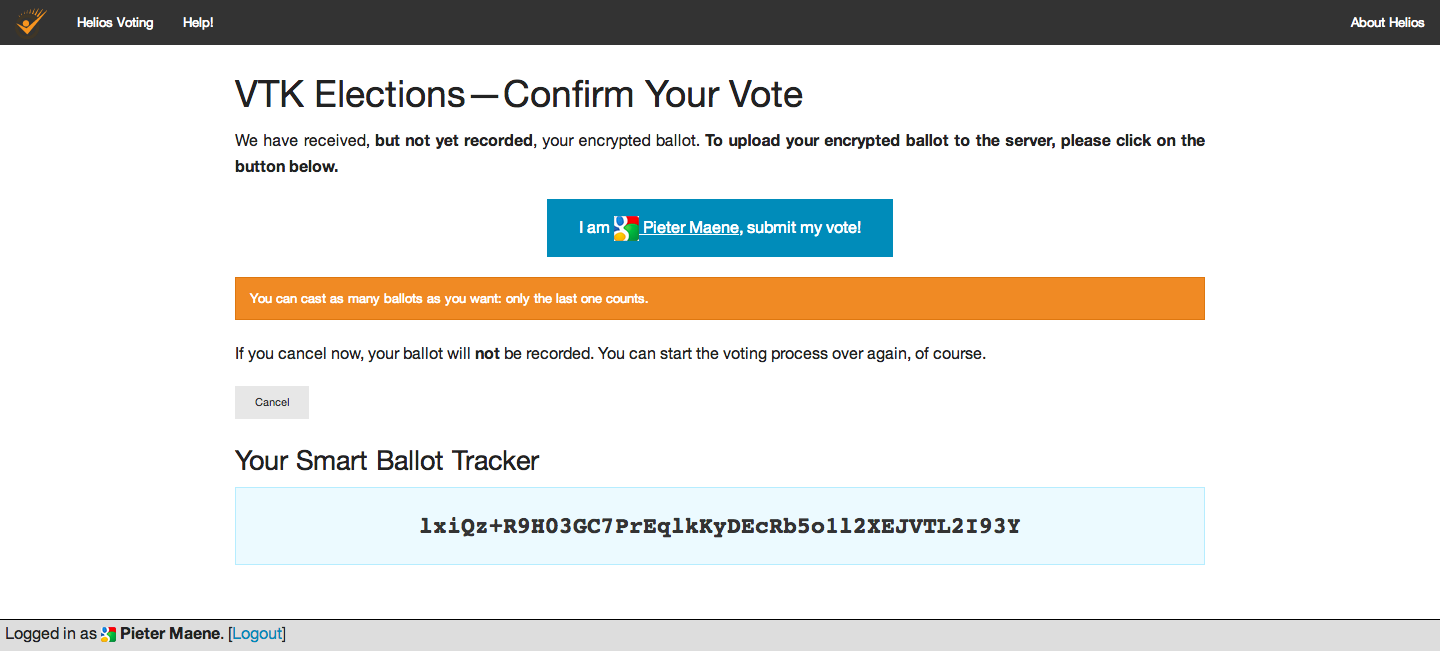
\includegraphics[width=\linewidth]{kv/cast_confirm.png}}
  \caption{Bevestigen van de stem}
  \label{fig:kv:cast_confirm}
\end{figure}

\subsection{Stresstest}

Er is elk jaar een opkomst van ongeveer 25\% bij de kringverkiezing van VTK, wat iets minder dan \np{1000} kiezers zijn. Daarom werd nagegaan of Helios ook een groot aantal stemmen nog correct kon verwerken. Hiervoor werd een aparte verkiezing aangemaakt met twee trustees en drie vragen. Vervolgens werden \np{1000} stemmen uitgebracht. Het resultaat kon van de eerste keer correct gedecrypteerd worden, dus hier was geen verdere actie nodig.

\npar Deze stemmen werden gegenereerd door een server-side actie. De kiezers stemmen normaal via het stemhokje, maar dat proces is moeilijk te automatiseren. Het grote verschil is dat de encryptie in Python in plaats van JavaScript gebeurt.

%TODO Remove Color

\npar \textcolor{blue}{Deze test werd niet op de server maar lokaal uitgevoerd. Het doel was hierbij te kijken of decryptie ook bij een groot aantal stemmen correct functioneerde. De belasting op de server van een groot aantal kiezers werd niet onderzocht omdat iedere kiezer slechts een beperkt aantal lichte requests uivoert.}

\section{Stemdag}
\label{sec:kv:stemdag}

De stemming zelf vond plaats op donderdag 8 mei 2014. Oorspronkelijk stond ze open van 7u00 tot 19u00. Omdat de communicatie 's ochtends traag op gang gekomen was, werd dit verlengd tot 20u00, wat ondersteund wordt door Helios. De trustees en het threshold schema waren dezelfde als tijdens de test (\ref{sec:kv:beheer}). De vragen en het resultaat worden getoond in \ref{fig:kv:result}. In totaal hebben 768 mensen hun stem uitgebracht, wat niet significant minder is dan in andere jaren. Dit is dus een sterke indicatie dat het proces voldoende eenvoudig is. Zowel bij het stemmen als het decrypteren van het resultaat waren er geen problemen.

\begin{figure}
  \center{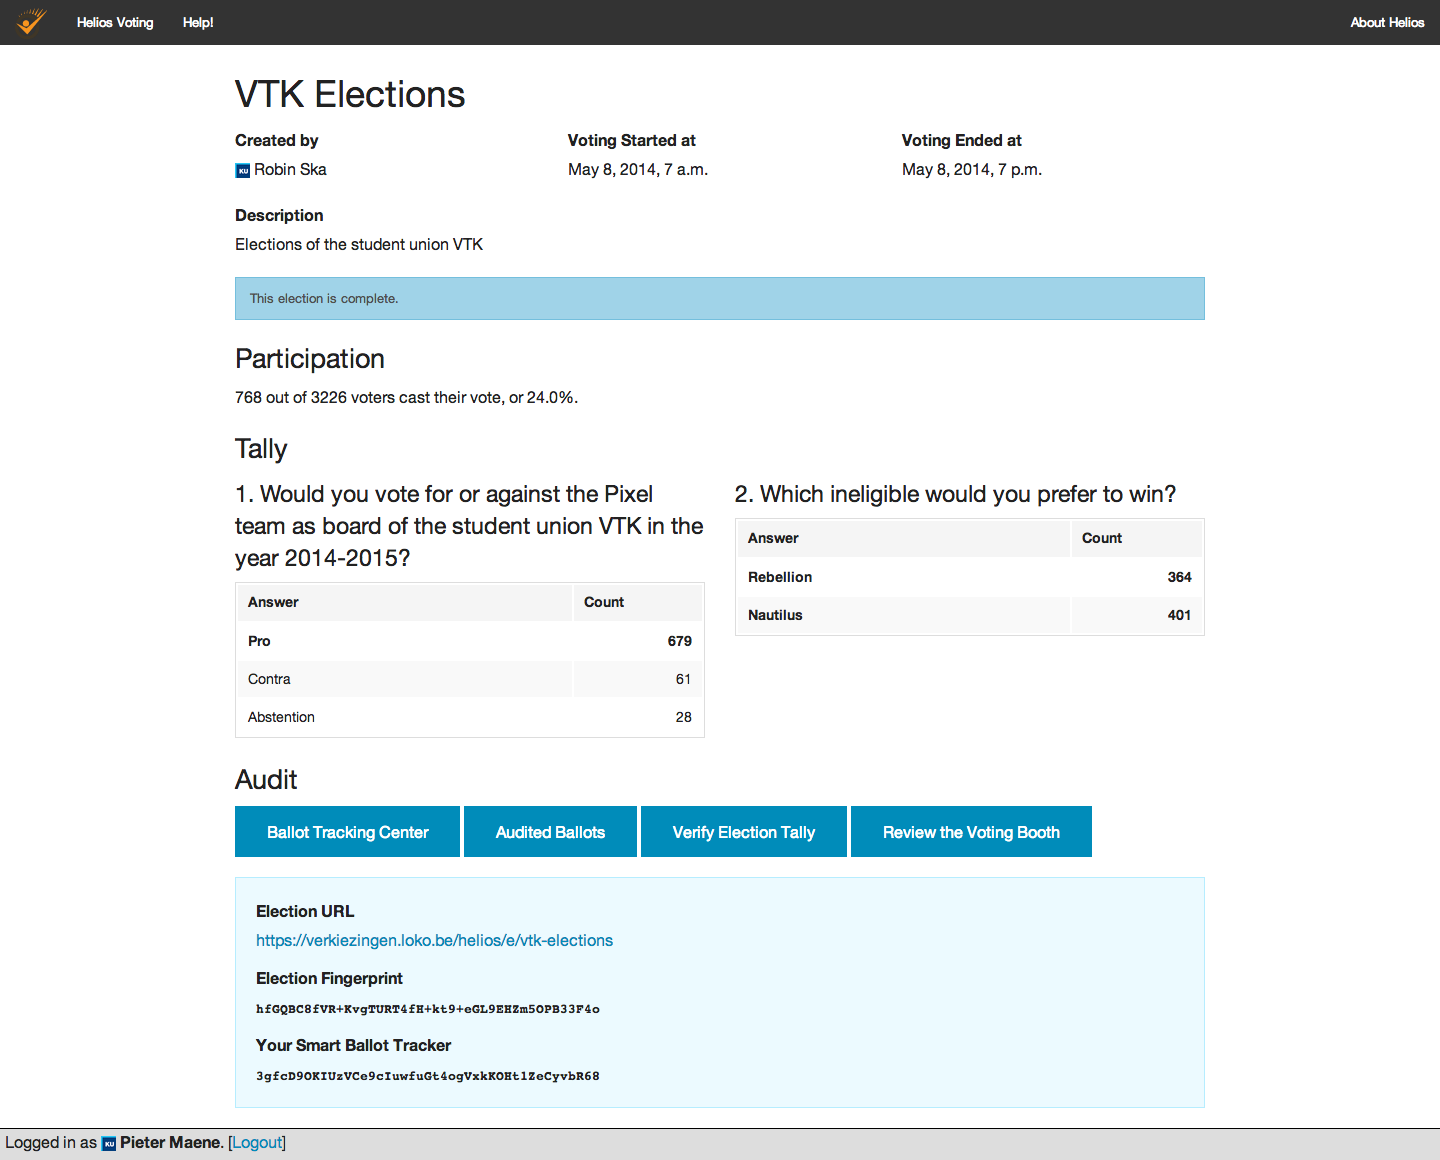
\includegraphics[width=\linewidth]{kv/result.png}}
  \caption{Resultaat van de stemming}
  \label{fig:kv:result}
\end{figure}

  % 
% Sleutels en Fingerprints
% @author Pieter Maene <pieter.maene@student.kuleuven.be>
%

\chapter{Bewaren van sleutels en fingerprints}
\label{chap:sleutels_en_fingerprints}

%TODO Remove Color

Tijdens de sleutelceremonie generen de trustees sleutelparen, waarvan de sleutels uiteraard veilig bewaard moeten kunnen worden (\ref{sec:sf:sleutels}). Daarnaast werkt Helios op verschillende plaatsen met fingerprints. In \ref{sec:sf:fingerprints} wordt eerst hun doel besproken, waarna gekeken wordt naar alternatieve methoden om ze weer te geven. \textcolor{blue}{Voor beide werden deze oplossingen theoretisch onderzocht, maar niet ge\"implementeerd.}

\section{Sleutels}
\label{sec:sf:sleutels}

\subsection{Disk}
\label{sec:sf:disk}

De trustees downloaden hun geheime sleutels als JSON bestanden (\ref{sec:ui:trustee_dashboard}). Deze zullen dus eerst bewaard worden op de harde schijf van de computer die op dat moment gebruikt wordt. Hier zijn twee belangrijke nadelen aan. Ten eerste zou iedereen die toegang heeft tot die machine de sleutel kunnen bemachtigen. Ten tweede kan de sleutel alleen vanaf deze machine gebruikt worden.

\npar Een eenvoudige oplossing voor het eerste probleem is de trustees vragen om hun account zeker te beveiligen met een wachtwoord. De sleutel zou ook op een beveiligde partitie geplaatst kunnen worden. Dit kan bijvoorbeeld gedaan worden door gebruik te maken van TrueCrypt.\cite{site:truecrypt}

\npar Wanneer de sleutel op een andere machine ingevoerd moet worden, kan deze op een USB-stick opgeslagen worden. Hier is het zeker aangeraden om de sleutel op een ge\"encrypteerde partitie te plaatsen. Daarnaast zou de sleutel ook ge\"upload kunnen worden naar een private server of een cloud opslagdienst. In dit geval moet hij zeker eerst ge\"encrypteerd worden.

\npar Het zou echter veel gebruiksvriendelijker zijn om dit in de generator in te bouwen. Voordat de sleutel gedownload wordt, kan deze eerst symmetrisch ge\"encrypteerd worden met een wachtwoord. Hiervoor zou bijvoorbeeld AES-CTR gebruikt kunnen worden, waarbij de sleutel afgeleid wordt van het opgegeven wachtwoord.\cite{rfc2898} Er zijn verschillende JavaScript libraries die hiervoor ondersteuning hebben.\cite{site:github_aes_js}\cite{site:github_sjcl} Bovendien wordt deze mode ook ondersteund door de Web Cryptography API (\ref{chap:web_cryptography_api}).\cite{sleevi_watson_web_cryptography_api}

\subsection{Web Storage~\cite{hickson_web_storage}\cite{site:pilgrim_local_storage}}
\label{sec:sf:web_storage}

Door gebruik te maken van de HTML5 Web Storage specificatie, zouden de sleutels ook op een alternatieve manier bewaard kunnen worden. Deze specificatie geeft een ontwikkelaar onder andere toegang tot een persistente key/value store waar tot 5MB aan data in opgeslagen kan worden. Er wordt ook voldaan aan de same-origin policy. Dit wil zeggen dat de data alleen toegankelijk zijn van op hetzelfde domein.\cite{gollman_computer_security}

\npar Deze functionaliteit zou toelaten om de geheime sleutels volledig te verbergen voor de trustees. In plaats van hen een bestand te laten downloaden met de sleutels, worden deze in de \texttt{localStorage} opgeslagen. Aangezien er naast de same-origin policy geen beveiligingsmechanismen ingebouwd zijn in de specificatie, is het beter om de sleutel eerst te encrypteren (\ref{sec:sf:disk}). Een \texttt{secureStorage} binnen de browser met ingebouwde encryptie zou dit nog eenvoudiger maken voor een ontwikkelaar.\cite{site:zakas_securestore} Een groot nadeel aan deze oplossing is dat de sleutel vast zit in de machine die gebruikt is om hem aan te maken.

\section{Fingerprints}
\label{sec:sf:fingerprints}

%TODO Explain SHA-256?

Op verschillende plaatsen binnen Helios worden fingerprints gebruikt. Dit zijn base64-ge\"encodeerde SHA-256 hashes van specifieke data. Zo is de \textit{Smart Ballot Tracker} (\ref{fig:kv:cast_confirm}) een fingerprint van de ge\"encrypteerde stem. Aan de trustee wordt ook een fingerprint van de gegenereerde publieke sleutels getoond. Dit zijn echter lange strings zijn die moeilijk te onthouden kunnen worden. Bovendien kan niet in \'e\'en oogopslag gezien worden of twee fingerprints hetzelfde zijn.

\npar Daarom kunnen hiervoor beter visuele hashes gebruikt worden. Dit zijn unieke afbeeldingen op basis van een bepaalde string. Afbeeldingen kunnen niet alleen sneller herkend worden, het is ook veel eenvoudiger om ze te bewaren. Wanneer de fingerprint een string is, moet deze neergeschreven worden of gekopieerd worden naar een bestand. Een afbeelding daarentegen kan eenvoudig gedownload worden. Voorbeelden van dergelijke visuele hashsystemen zijn RoboHash (\ref{fig:sf:robohash}) en Identicon.\cite{site:robohash}\cite{wiki:identicon}

%TODO Remove Color

\npar \textcolor{blue}{Een belangrijke voorwaarde voor het stemhokje is dat er geen netwerk requests meer mogen gebeuren voordat de stem volledig ge\"encrypteerd is.\cite{adida_helios} In het aangepaste stemhokje wordt het biljet ge\"encrypteerd nadat alle keuzes gemaakt zijn. Hoewel deze voorwaarde dus voldaan is wanneer de fingerprint getoond wordt, moet toch de voorkeur gegeven worden aan een systeem dat de figureren lokaal kan genereren. Indien een JavaScript implementatie niet mogelijk is, zouden ze gedownload kunnen worden van de server over een beveiligde verbinding.}

\begin{figure}
  \center{
\includegraphics[width=0.5\linewidth]{sf/robohash.png}}
  \caption{RoboHash van de fingerprint in \ref{fig:kv:cast_confirm}}
  \label{fig:sf:robohash}
\end{figure}

  % 
% Web Cryptography API
% @author Pieter Maene <pieter.maene@student.kuleuven.be>
%

\chapter{Web Cryptography API}
\label{chap:web_cryptography_api}

Wanneer webontwikkelaars vandaag cryptografische functies nodig hebben in hun toepassingen, moeten ze bijna JavaScript gebruiken omwille van compatibiliteit. Hoewel er de laatste jaren zeer grote vooruitgang geboekt is, zullen de meeste JavaScript engines nog steeds minder goed presteren dan native code.\cite{site:resig_javascript_performance_rundown}\cite{site:cois_javascript_performance_rundown_2012}\cite{smedberg_performance_analysis_of_javascript} De W3C startte in 2012 een working group op om een nieuwe browser API te defini\"eren: de Web Cryptography API.\cite{wiki:webcrypto}

\npar In \ref{sec:wc:web_cryptography_api} wordt deze nieuwe API kort besproken. Daarna wordt in \ref{sec:wc:nfwebcrypto} gekeken naar de NfWebCrypto polyfill, die de nieuwe functionaliteit implementeert in een plugin voor Google Chrome. Tot slot wordt deze implementatie in \ref{sec:wc:benchmarks} vergeleken met bestaande cryptografische libraries.

\section{Web Cryptography API~\cite{sleevi_watson_web_cryptography_api}}
\label{sec:wc:web_cryptography_api}

De Web Cryptography API definieert cryptografische operaties die gebruik maken van sleutels die beheerd worden door de browser. Al deze methodes zitten in de \texttt{SubtleCrypto} interface. Er zijn zowel methodes voor het beheren van het sleutelmateriaal als het encrypteren van data.

\npar De API is ontworpen vanuit het idee om alleen standaardfunctionaliteit aan te bieden. Er wordt dus maar een beperkt aantal algoritmes ondersteund, die bovendien elk nog vaak hun eigen beperkingen hebben.\cite{mail:sleevi_algorithms_and_referenced_documents} Naargelang de functionaliteit van het algoritme, ondersteunt ook niet elk algoritme alle methodes van de interface.

\section{NfWebCrypto}
\label{sec:wc:nfwebcrypto}

Aangezien de standaard nog niet voltooid is, wordt deze nauwelijks ondersteund door de grote browsers.\cite{site:html5test_web_cryptography_api} Alleen Internet Explorer 11 heeft reeds een implementatie, maar hierin is slechts een beperkt aantal algoritmes aanwezig.\cite{site:microsoft_web_cryptography} Om de vergelijking met de andere JavaScript libraries toch te kunnen uitvoeren, was dus een alternatieve implementatie nodig van deze API.

\npar PolyCrypt is een JavaScript polyfill ontwikkeld door BBN Technologies.\cite{site:polycrypt} Een polyfill implementeert een browser API die (nog) niet native ondersteund wordt. Omdat deze gebaseerd is op een oudere draft van de API, miste ook hierin functionaliteit die nodig was voor de tests. Een bijkomend nadeel aan deze implementatie is dat ze in JavaScript geschreven is, waardoor een eventueel snelheidsvoordeel ten opzichte van de andere libraries waarschijnlijk niet naar voor zou komen.

\npar NfWebCrypto daarentegen is een \cplusplus polyfill ontwikkeld door Netflix.\cite{site:nfwebcrypto} Intern wordt de bekende OpenSSL library gebruikt voor de cryptografische functionaliteit. Het grote voordeel is hier dus dat de cryptografische code nu native is, waardoor de prestaties vergelijkbaar zouden moeten zijn met die van een echte implementatie in de browser. Het grootste nadeel is hier wel dat het een plugin is voor Chrome. Bovendien moet deze handmatig gecompileerd worden en moet de browser op een speciale manier gestart worden, zodat het gebruik ervan niet zo vanzelfsprekend is. Hoewel dit dus gebruikt kan worden voor de tests, is dit niet direct bruikbaar voor praktische applicaties.

\section{Benchmarks}
\label{sec:wc:benchmarks}

\subsection{Modulaire exponentiatie}
\label{sec:wc:modulaire_exponentiatie}

Helios maakt gebruik van ElGamal (\ref{sec:helios:elgamal}) om de stemmen te encrypteren. Dit algoritme wordt echter niet ondersteund door de Web Cryptography API (\ref{sec:wc:web_cryptography_api}). Deze kan dus niet onmiddellijk gebruikt worden om de encryptie te versnellen. De modulaire exponentiaties vragen veruit de meeste rekentijd. Een verbetering daar zou dus ook positief zijn voor de algemene prestaties.

\npar Aangezien de enige publieke methodes van de API op hoog niveau werken, is er geen functie beschikbaar om dit te doen. Diffie-Hellman wordt echter wel ondersteund voor het genereren van een assymmetrisch sleutelpaar. De \texttt{deriveKey} methode van de API berekent de gedeelde geheime sleutel volgens \ref{eq:wc:diffie_hellman}.\cite{diffie_hellman_new_directions_in_cryptography}

\begin{equation}
  \label{eq:wc:diffie_hellman}
  K = (g^a)^b \mod{p}
\end{equation}

\npar Hier is $g^a$ de publieke sleutel van A en b de geheime sleutel van B.  Om de modulaire exponentiatie $x^y \mod{p}$ uit te rekenen, moet het dus mogelijk zijn om de publieke sleutel $g^a$ gelijk te stellen aan $x$ en de geheime sleutel aan $y$.

\npar Om een specifieke geheime sleutel te kunnen gebruiken in de \texttt{deriveKey} methode, moet deze eerst ge\"importeerd worden in de key store. Hiervoor kan de \texttt{importKey} methode gebruikt worden. Samen met de naam van het algoritme (DH) worden als parameters de geheime sleutel, het priemgetal $p$ en de generator $g$ meegegeven. De standaard laat het importeren van de geheime sleutel alleen toe wanneer deze het $PKCS8$ formaat heeft.\cite{rfc5208} Om de testen te vereenvoudigen, werd de NfWebCrypto plugin aangepast om het importeren van ruwe geheime sleutels toch mogelijk te maken.

\npar Daarna kan de modulaire exponentiatie uitgerekend worden door \texttt{deriveKey} aan te roepen met $x$ als argument voor de publieke sleutel. Na het afleiden wordt de gemeenschappelijke sleutel opnieuw opgeslagen in de key store. Ook hier waren enkele kleine aanpassingen nodig aan de code van de plugin om het berekenen van de geheime sleutel met onze eigen waarden mogelijk te maken. De \texttt{exportKey} methode kan tot slot gebruikt worden om het ruwe resultaat te exporteren. 

\npar De prestaties van NfWebCrypto worden vergeleken met deze van JSBN en Leemon, twee big number libraries die geschreven zijn in JavaScript.\cite{site:wu_rsa_and_ecc_in_javascript}\cite{site:baird_big_integers_in_javascript} Er wordt telkens een exponent van \np{1024} bit gebruikt, wat ook de lengte van de parameters in Helios is. De berekening werd voor elke library \np{1000} keer uitgevoerd om een statistisch relevant resultaat te bekomen. De resultaten worden weergegeven in \ref{fig:wc:modular_exponentiation} en \ref{tab:wc:modular_exponentiation}. De berekening duurt bij Leemon veruit het langste. De JSBN library is sterk geoptimaliseerd. De NfWebCrypto plugin is daarentegen gemiddeld nog eens dubbel zo snel. De variantie is hier zo groot omdat de eerste exponentiatie veel langer duurt.

\npar Het resultaat dat bekomen wordt na de \texttt{exportKey} is wel niet correct. In de communicatie met de plugin moeten de parameters \texttt{base64} ge\"encodeerd worden. Vermoedelijk loopt hier nog iets mis tussen de conversie in JavaScript en \cplusplus.

\begin{figure}
  \center{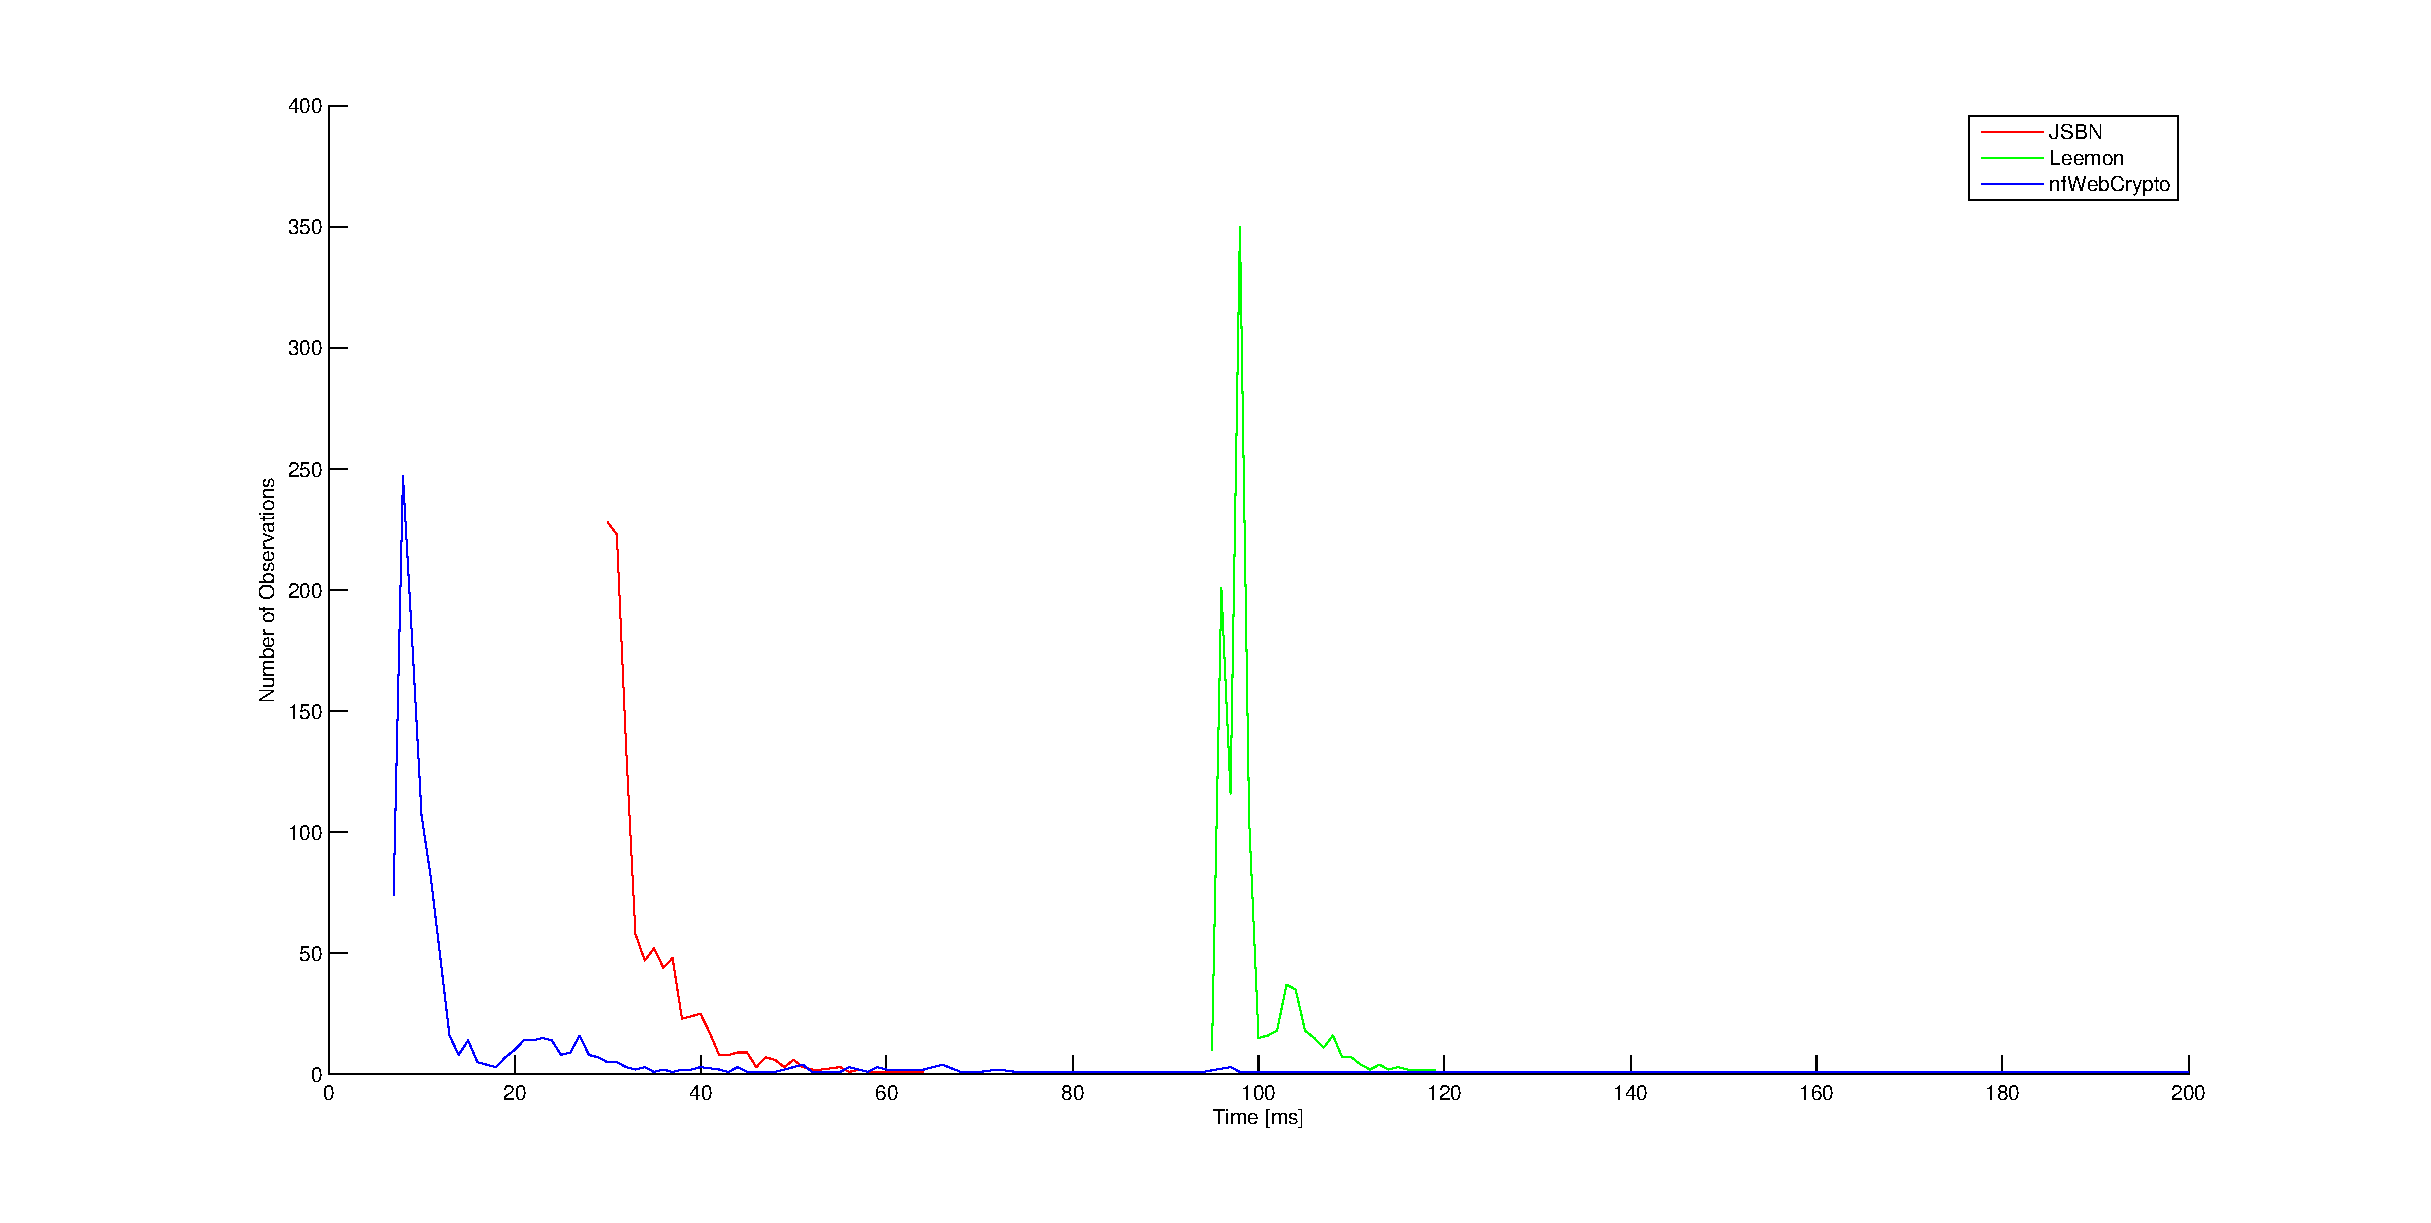
\includegraphics[width=\linewidth]{wc/modular_exponentiation.eps}}
  \caption{Modulaire exponentiatie}
  \label{fig:wc:modular_exponentiation}
\end{figure}

\begin{table}
  \begin{center}
    \begin{tabular}{r | c c}
      Library & Gemiddelde [ms] & Variantie [ms] \\ \hline
      JSBN & 33,9250 & 26,5019  \\
      Leemon & 99,1470 & 15,0785 \\
      NfWebCrypto & 16,0670 & 470,6251
    \end{tabular}
    \caption{Modulaire exponentiatie}
    \label{tab:wc:modular_exponentiation}
  \end{center}
\end{table}

\subsection{RSA}

Een tweede vergelijking werd gemaakt tussen JSBN en NfWebCrypto voor een RSA encryptie. Dit wordt niet gebruikt in Helios, maar ook deze resultaten zijn zeer interessant. De berekening van de RSA cijfertekst is opnieuw een modulaire exponentiatie (\ref{eq:wc:rsa}).\cite{rivest_shamir_adleman_rsa}

\begin{equation}
  \label{eq:wc:rsa}
  c = m^e \mod{n}
\end{equation}

\npar Hier is het paar $(n, e)$ de publieke sleutel van de partij waarvoor het bericht ge\"encrypteerd wordt. Voor de publieke exponent $e$ werd de standaardwaarde \np{65537} genomen. Merk op dat deze heel wat korter is dan de \np{1024}-bit exponenten die in de tests van \ref{sec:wc:modulaire_exponentiatie} gebruikt werden. De lengte van de modulus is \np{1024} bit.

\npar De JSBN library voorziet in enkele klassen specifiek voor RSA encryptie en decryptie. Het is dus zeer eenvoudig om een bepaalde klaartekst te encrypteren met een gegeven publieke sleutel. De Web Cryptography API ondersteunt hier het \texttt{RSAES-PKCS1-v1\_5} algoritme voor.\cite{rfc3447} Hoewel het mogelijk zou moeten zijn om publieke sleutels in het \texttt{SPKI}-formaat te importeren, bleek het opnieuw moeilijk om de sleutel die gebruikt werd voor de JSBN encryptie om te zetten. Daarom werd besloten om voor elke encryptie een nieuwe sleutel te genereren. De tijd die hiervoor nodig is, wordt niet meegerekend in het eindresultaat.

\npar Ook hier werd de encryptie \np{1000} keer uitgevoerd. De resultaten van deze test zijn terug te vinden in \ref{fig:wc:rsa} en \ref{tab:wc:rsa}. We zien dat de JavaScript implementatie voor deze veel kortere exponent sneller is dan de berekening door de NfWebCrypto plugin. De communicatie met de plugin weegt hier duidelijk zwaarder door.

\begin{figure}
  \center{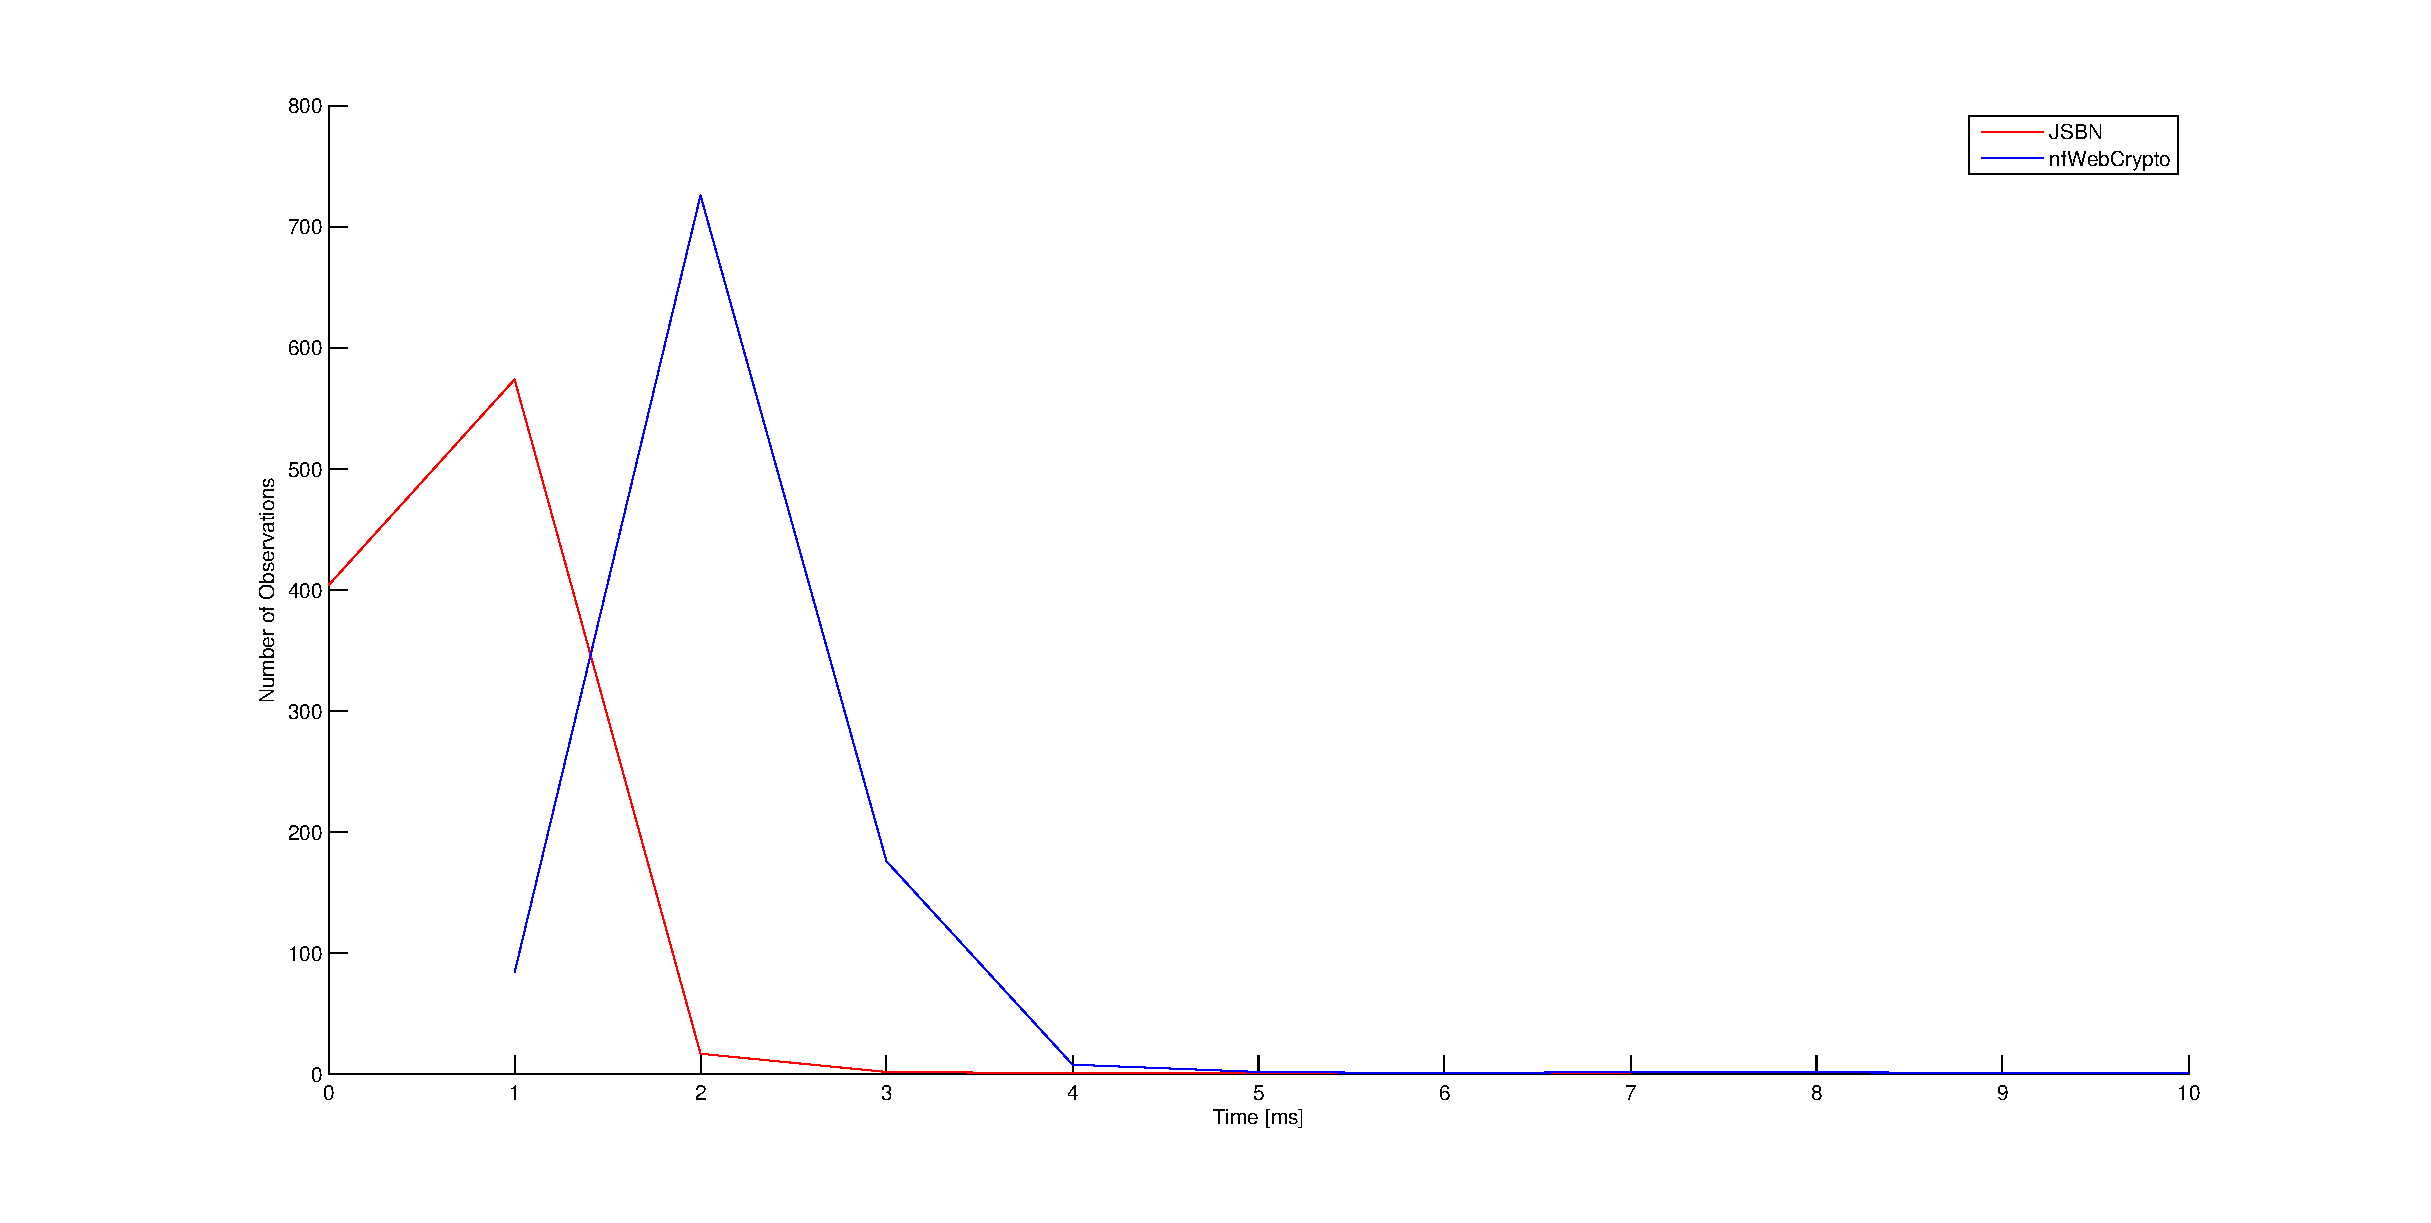
\includegraphics[width=\linewidth]{wc/rsa.eps}}
  \caption{RSA}
  \label{fig:wc:rsa}
\end{figure}

\begin{table}
  \begin{center}
    \begin{tabular}{r | c c}
      Library & Gemiddelde [ms] & Variantie [ms] \\ \hline
      JSBN & 0,6310 & 0,3632  \\
      NfWebCrypto & 2,1360 & 0,4219
    \end{tabular}
    \caption{RSA}
    \label{tab:wc:rsa}
  \end{center}
\end{table}

\section{Besluit}

Dankzij de Web Cryptography API zal het eenvoudiger worden om cryptografie te gebruiken in de browser. Bovendien is er een merkbare snelheidswinst ten opzichte van de huidige JavaScript implementaties, wat belangrijk is voor de gebruiksvriendelijk. 

\npar Dat slechts een beperkt aantal algoritmes ondersteund wordt, is een belangrijk nadeel van de API. Omdat de methodes die publiek beschikbaar zijn op een hoog niveau werken, is het zeer moeilijk om deze te gebruiken voor het versnellen van alternatieve algoritmes.

\npar Daarnaast was het ook ingewikkeld om sleutels die buiten de plugin gegenereerd waren, correct te importeren. Dit werd echter voornamelijk veroorzaakt door de encoding van de communicatie en is dus niet noodzakelijk een inherent probleem van de API.

  % 
% Besluit
% @author Pieter Maene <pieter.maene@student.kuleuven.be>
%

\chapter{Besluit}
\label{chap:besluit}




  \appendix
  
  \chapter{English Paper}
  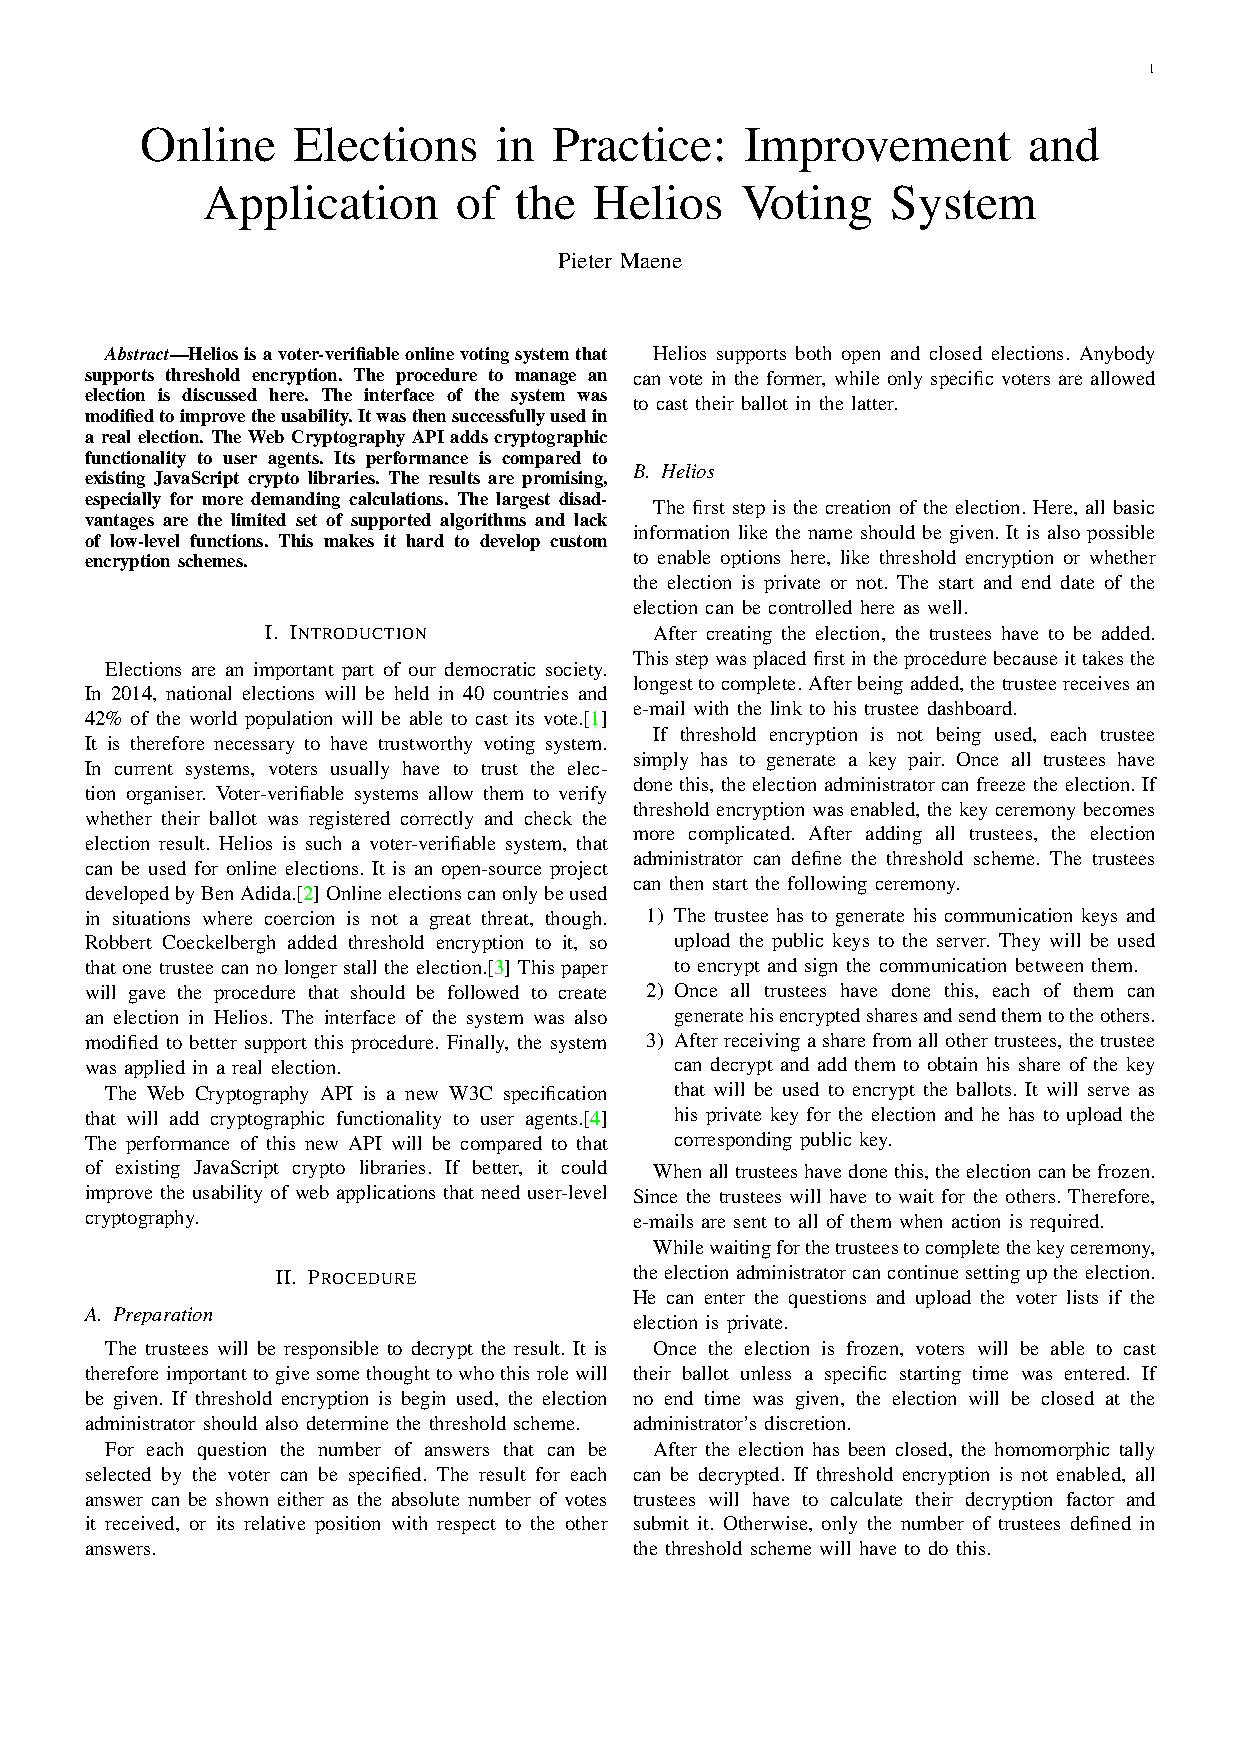
\includepdf[pages={-}]{../Paper/paper.pdf}

  \backmatter

  % Bibliography
  \nocite{*}

  \bibliographystyle{plain}
  \bibliography{references}

\end{document}
